% IWAI 2026 submission: Springer LNCS format, max 12 pages (incl. figures,
% excl. references) + appendix of up to 12 pages, double-blind.
\documentclass[runningheads]{llncs}

% ---------- encoding & fonts ----------
\usepackage[T1]{fontenc}
\usepackage[utf8]{inputenc}
\usepackage[expansion=false]{microtype}

% ---------- math ----------
\usepackage{amsmath}
\usepackage{amssymb}
\usepackage{mathtools}

% ---------- figures ----------
\usepackage{graphicx}
\graphicspath{{figures/}}
\usepackage{tikz}
\usetikzlibrary{calc,positioning,arrows.meta}
\usepackage{subcaption}
\usepackage{xcolor}

% ---------- layout ----------
% (LNCS fixes the text block; geometry must not be loaded)
\usepackage[numbers,sort&compress]{natbib}
\usepackage{hyperref}
\hypersetup{hidelinks}

% ---------- shorthands ----------
\newcommand{\KL}[2]{D_{\mathrm{KL}}\!\left[#1\,\middle\|\,#2\right]}
\newcommand{\E}[1]{\mathbb{E}\!\left[#1\right]}
\newcommand{\Eq}[2]{\mathbb{E}_{#1}\!\left[#2\right]}
\newcommand{\Var}[2]{\mathrm{Var}_{#1}\!\left[#2\right]}
\newcommand{\desc}{\mathrm{desc}}
\newcommand{\rw}{\rightsquigarrow}
\newcommand{\Top}{\mathsf{T}}          % propagation operator
\newcommand{\bone}{\mathbf{1}}         % unit source vector

% ---------- palette ----------
\definecolor{costc}{RGB}{40,80,170}
\definecolor{newc}{RGB}{200,120,30}      % proposed / new node (amber)

% ---------- network figure macros ----------
\tikzset{
  bel/.style={circle,draw=black!70,line width=0.4pt,minimum size=7mm,inner sep=0pt,font=\small},
  obs/.style={rectangle,draw=black!45,fill=white,minimum size=2.6mm,inner sep=0pt},
  core/.style={line width=0.9pt,black!75},
  belt/.style={line width=0.5pt,black!55},
  sens/.style={dashed,line width=0.4pt,black!40},
  anno/.style={font=\scriptsize\itshape,text=black!75,align=center},
  annoarrow/.style={-{Stealth[length=1.4mm]},line width=0.3pt,black!55},
  % directed dependency edges; the *c variants shorten to clear 7mm nodes drawn at coordinates
  dcore/.style={-{Stealth[length=1.5mm]},line width=0.9pt,black!75},
  dbelt/.style={-{Stealth[length=1.3mm]},line width=0.5pt,black!55},
  dcorec/.style={dcore,shorten <=0.37cm,shorten >=0.37cm},
  dbeltc/.style={dbelt,shorten <=0.37cm,shorten >=0.37cm},
}
\newcommand{\Positions}{%
  \coordinate (A) at (0,1.1);   \coordinate (B) at (-1.1,0);
  \coordinate (C) at (1.1,0);   \coordinate (D) at (0,-1.1);
  \coordinate (b1) at (-1.45,1.95); \coordinate (b2) at (1.45,1.95);
  \coordinate (b3) at (-2.25,0);    \coordinate (b4) at (2.25,0);
  \coordinate (b5) at (-1.45,-1.95);\coordinate (b6) at (1.45,-1.95);
  \coordinate (o1) at (-1.95,2.6);  \coordinate (o2) at (1.95,2.6);
  \coordinate (o3) at (-3.1,0);     \coordinate (o4) at (3.1,0);
  \coordinate (o5) at (-1.95,-2.6); \coordinate (o6) at (1.95,-2.6);
}
\newcommand{\Edges}{%
  \draw[dcorec] (A)--(B); \draw[dcorec] (A)--(C); \draw[dcorec] (A)--(D);
  \draw[dcorec] (B)--(C); \draw[dcorec] (B)--(D); \draw[dcorec] (C)--(D);
  \draw[dbeltc] (A)--(b1); \draw[dbeltc] (A)--(b2);
  \draw[dbeltc] (B)--(b3); \draw[dbeltc] (C)--(b4);
  \draw[dbeltc] (D)--(b5); \draw[dbeltc] (D)--(b6);
  \draw[sens] (b1)--(o1); \draw[sens] (b2)--(o2); \draw[sens] (b3)--(o3);
  \draw[sens] (b4)--(o4); \draw[sens] (b5)--(o5); \draw[sens] (b6)--(o6);
  \node[obs] at (o1){}; \node[obs] at (o2){}; \node[obs] at (o3){};
  \node[obs] at (o4){}; \node[obs] at (o5){}; \node[obs] at (o6){};
}
% tiny 3-node paradigm DAG inside an agent circle at (#1,#2)
\newcommand{\miniNet}[2]{%
  \draw[black!70,line width=0.5pt,fill=white] (#1,#2) circle (0.46);
  \fill[costc!75] ($(#1,#2)+(0,0.22)$) circle (0.055);
  \fill[costc!75] ($(#1,#2)+(-0.22,-0.13)$) circle (0.055);
  \fill[costc!75] ($(#1,#2)+(0.22,-0.13)$) circle (0.055);
  \draw[costc!80,line width=0.4pt,-{Stealth[length=1mm]}] ($(#1,#2)+(0,0.22)$) -- ($(#1,#2)+(-0.22,-0.13)$);
  \draw[costc!80,line width=0.4pt,-{Stealth[length=1mm]}] ($(#1,#2)+(0,0.22)$) -- ($(#1,#2)+(0.22,-0.13)$);
  \draw[costc!80,line width=0.4pt,-{Stealth[length=1mm]}] ($(#1,#2)+(-0.22,-0.13)$) -- ($(#1,#2)+(0.22,-0.13)$);
}

% ======================================================================
\title{Changing a Networked Mind: Paradigm Dynamics as Structure Learning over a Hidden World}
\titlerunning{Changing a Networked Mind}
% ----- ANONYMIZED for double-blind review. Restore for camera-ready: -----
% \author{Jonas Hallgren\inst{1} \and David Hyland\inst{2} \and Mahault Albarracin\inst{3}}
% \authorrunning{J. Hallgren et al.}
% \institute{Affiliation 1 \email{...} \and Affiliation 2 \and Affiliation 3}
\author{Anonymous Submission}
\authorrunning{Anonymous Submission}
\institute{Anonymous Institution(s)}
% ======================================================================

\begin{document}
\maketitle

\begin{abstract}
How does a scientific community change its mind---not about a fact, but about the \emph{frame} its
facts live in? We model a paradigm as a directed network of commitments and a community as bounded
active-inference agents who must \emph{learn} that network's structure while valuing some
conclusions over others and pooling beliefs with peers. Built from its field's default
choices---Gaussian beliefs, precision-weighted pooling---such a community provably cannot run the
Kuhnian cycle: conflict resolves into confident compromise, any contact forces consensus, and the
lone discoverer of a new dimension is averaged away. We then add the one quantity whose absence
those theorems name: \emph{reliability, inferred from surprise}---each agent trusts what does not
keep surprising it, applying the same Student-$t$ weight $\lambda=(\nu+1)/(\nu+z^2)$ to its own
sensory channels and to its peers. This single gate generates the missing phenomenology
endogenously: the community doubts its instruments before its theory (denial), holding the old
paradigm at a fraction of the un-gated conversion rate and rehabilitating the channels it
condemned; conflict registers as suspended confidence rather than growing certainty; communities
sever trust, persist as schools past a sharp incommensurability threshold set by the confidence
each accumulated apart, and re-merge through a distrust--plateau--rehabilitation arc whose
ending, unlike its onset, is fast---the reopening gate accelerates its own reopening. Everything the gate buys is a
\emph{timescale}, not a wall: consensus remains the only fixed point, moved out of reach. And a
pluralism of frames survives contact only when trust reads the \emph{wiring} of a peer's beliefs,
not their opinions. Open-endedness in a community of structure learners is a property of its
pooling protocol---designed in, never an emergent grace of scale.

\keywords{Active inference \and Structure learning \and Belief sharing \and Paradigm change \and Social epistemology}
\end{abstract}

% ======================================================================
\section{Introduction: changing a frame, not a credence}
\label{sec:background}
% ======================================================================

If we want science to keep going well, goodwill is not enough: we need to know how science
\emph{works}---what kind of agent can do science at all, how a community comes to represent a
genuinely new dimension of the world, and how it loses information it once held. The question has
lately acquired a second audience, because communities of reasoning agents are no longer only
studied but \emph{built}---machine-mediated research pipelines, automated literature synthesis,
multi-agent learning systems---and every such community commits, in its aggregation step, to an
answer it rarely examines: what happens to the member who disagrees. Machine learning has begun
to name the property at stake \emph{open-endedness}, the capacity of a system to keep producing
artifacts that are novel and learnable, identified both as a grand challenge
\citep{stanley2017oe} and as an essential ingredient of any general intelligence
\citep{hughes2024}; social epistemology has long catalogued its failure modes, echo chambers
\citep{nguyen2018} and premature consensus \citep{zollman2010}. What neither supplies is a
foundation: a model of a \emph{community} of structure-learning agents explicit enough that one
can prove which aggregation dynamics preserve open-endedness and which foreclose it. This paper
builds that foundation and gives the question both halves of an answer. The most natural
baseline---Gaussian beliefs under precision-weighted pooling---provably lacks the capacity:
averaging refines a frame; it cannot grow a new one. And the cheapest repair the failure itself
names---making each source's \emph{reliability} a quantity inferred from surprise rather than a
constant---restores the missing dynamics wholesale, at a price the model makes precise: every
protection it buys is a timescale, never a wall.

To change one's mind about a fact is to update a belief; to change a paradigm is to change the
\emph{frame} in which beliefs are posed. A frame is not a credence but a \emph{structure}: a
network of conditional dependencies through which information propagates. A community that revised
only its credences, leaving the network fixed, could never change frame at all. This is the
phenomenon Kuhn named but could not run forward \citep{kuhn1962}: nothing in \emph{The Structure of
Scientific Revolutions} says, mechanistically, why a community holds a structure of commitments
long past the first disconfirming evidence, nor what finally makes the holding give way.

When the chemical community gave up phlogiston it did not revise a single credence. It rewrote a
network of commitments in which combustion, calcination, respiration, and the theory of acids were
all load-bearing on a hub that had to go: late-phlogistic theorists proposed cascading revisions that
proved mutually incompatible \citep{blumenthal2017,holmes2000}, defending less a hypothesis about
combustion than a constellation of entangled commitments \citep{boantza2011}. Phlogiston was
load-bearing for too much.

Network epistemology, the dominant formalism for such communities, cannot represent this case. Its
agents hold a scalar credence in a fixed proposition and update it on a trust graph
\citep{zollman2010,oconnor2019,zollman2013}---a programme with striking results on transient
diversity, polarization, and the division of cognitive labour
\citep{jonard2025,michelini2023,kitcher1990,strevens2003}, but the phlogiston puzzle is not a failure
to converge on a number. The commitments were \emph{entangled}: revising one forced a re-reading of
the others, and the dispute was over which entanglements to keep. Thagard's ECHO
\citep{thagard1989,thagard1990} captures the structural intuition as undirected coherence, but lacks
the directed dependencies, the carry-over cost of mind-change, and the expand/reduce asymmetry we
derive below. Active-inference accounts supply an endogenous, precision-based lock-in mechanism
\citep{albarracin2022} and warn that naive aggregation degrades collective precision
\citep{friston2023federated,waade2025}; the variational cost of mind-change has been formalized for a
single agent as a motivated trade between revision cost and the utility of a held belief
\citep{hyland2025}. What none of these does is make \emph{belief structure itself} the object of
inference. A scalar credence over a fixed menu of hypotheses cannot say how revising one commitment
forces a re-reading of the rest, nor how a community arrives at a \emph{new} way of carving up the
world: its members can herd on a number or split over it, but they can never come to hold different
\emph{kinds} of world---only different values on a shared one.

This paper lets a piece of \emph{structure} travel, so that one agent can come to represent a
commitment its peers do not. Its agents carry a directed network of commitments and learn that
network by Bayesian model expansion and reduction; they are \emph{bounded}, sampling a complex
world through narrow channels, valuing some conclusions over others, and judging what they
receive against their own model. Section~\ref{sec:bmebmr} assembles this community from the
field's own default choices, states the two classical theorems under which those defaults can
neither reject a conflicting source nor sustain a school---so that \emph{conflict resolves into
confident compromise}, and the Kuhnian cycle provably cannot run---and then equips every agent
with the one inference the theorems forbid the defaults: reliability, read off surprise, applied
alike to the agent's own instruments and to its neighbours.
Section~\ref{sec:results} drives the gated community through the full cycle---normal science,
anomaly, denial, crisis, discovery, schism, rehabilitation---and measures what one inferred
quantity buys and what it still cannot. The story, compactly, is about averaging---what belief
revision is when value enters as a tilt rather than a stiffness, what propagation-by-averaging
does to a population of structure learners, and what it takes for multi-agent structure learning
to be \emph{open-ended} rather than self-sealing.

% ======================================================================
\section{What a model of science must contain}
\label{sec:hidden}
% ======================================================================

Three things, at least. \emph{Structure as the object of inference}: a scientist confronting a
new domain is not given the right variables, let alone the dependencies among them---whether two
regularities share a hidden common cause, are lawfully coupled, or merely coincide is exactly
what she must learn. Frames differ in kind, not in degree, so credences over a fixed menu cannot
carry them; the theory-acquisition literature reaches the same conclusion, casting conceptual
development as a stochastic search over structures \citep{ullman2020,kemp2008form,ullman2012}.
Once structure is the object, exploration stops being a hand-tuned bonus---an $\epsilon$, a
temperature, a switching cost \citep{zollman2010,oconnor2019}---and becomes the epistemic value
of \emph{expanding} the model to entertain a commitment not yet in it
\citep{friston2015,friston2017curiosity}, with Bayesian model reduction as its complement,
pruning what the data abandon in closed form \citep{friston2018bmr,neacsu2022}. Existing
applications of that machinery run on single agents \citep{neacsu2022,priorelli2023} or define
``group'' as between-subject neuroimaging \citep{friston2016peb}; a \emph{community} jointly
expanding and reducing a paradigm is the open move this paper makes.

\emph{Value}, because scientists care about their conclusions: a result on which a career rests
is held more tightly than its evidence warrants \citep{kitcher1990,strevens2003}, and attitudes
demonstrably live on networks of exactly this kind \citep{dalege2016}. And \emph{communication},
because science is social: beliefs travel a trust graph and must somehow be combined when they
meet. Each requirement has a default formalization, so natural it is hardly ever examined.
Beliefs over a network become a precision-weighted Gaussian model; value becomes a utility that
tilts the posterior \citep{hyland2025}; combination becomes precision-weighted averaging, the
information form of classical opinion pooling \citep{degroot1974,genest1986}. And hiding inside
the third is a fourth default, so quiet it is rarely stated: the \emph{weights} of the
averaging---how much an agent trusts each instrument and each peer---are constants, blind to what
the source actually says. Section~\ref{sec:bmebmr} builds the community out of exactly these
defaults, on purpose, and then revokes only the fourth: reliability becomes something an agent
\emph{infers}. The question the rest of the paper asks is what that single change buys---whether
agents built this way can grow a frame, hold a school, and lose a paradigm, and not merely polish
the frame they have.

% ======================================================================
\section{The model}
\label{sec:bmebmr}
% ======================================================================

We build the object up from the single agent and then state the population dynamics as an explicit
per-round loop (\S\ref{sec:model}).

\subsection{A paradigm network and its operator}
\label{sec:carryover}

Begin concretely. The phlogiston paradigm, at its smallest, is three commitments wired together:
combustion releases phlogiston; calcination is combustion, slowed; respiration is combustion,
tamed. Each commitment conditions the next, evidence for any one bears on all, and the question
``what if the calx \emph{gains} weight?'' has no local answer---it tugs the whole web. A
paradigm, in this paper, is that web made explicit.

An agent represents a paradigm as a directed network $G=(V,E,\Pi)$: nodes carry theoretical
commitments $x_v$, edges carry inferential dependencies, and each edge bears a coupling precision
$\pi_{uv}$ measuring how tightly $v$ is bound to $u$. This is just a generative model whose hidden
states are the commitments themselves, with precision playing its usual role: a high-$\pi$ edge says
that belief in $u$ strongly constrains belief in $v$. Internal coherence is the corresponding
precision-weighted graphical model, $p(x\mid G)\propto\prod_{(u\to v)\in
E}\psi_{uv}(x_u,x_v)^{\pi_{uv}}$. None of this machinery is ours: it is a linear-Gaussian structural
equation model in the lineage of Wright's path analysis \citep{wright1934}, edges as path
coefficients and precisions as their weights. We work
throughout in that \emph{linear-Gaussian} regime, which puts every quantity below in closed form
(Appendix~\ref{app:operator}); agents are \emph{honest}---no one misreports, so lock-in is never a
dishonesty artifact---and \emph{bounded}, minimizing variational free energy step by step
\citep{dacosta2020} rather than planning over policies.

Revising a commitment is not a local act: changing $x_v$ forces everything downstream to
re-equilibrate, along every chain of dependence. If $A$ is the matrix of edge precisions, $A^k$
collects the chains of length $k$, and summing chains of every length gives
$\sum_k A^k=(I-A)^{-1}$---a finite sum on a DAG. Two literatures already own this object: path
analysis as the \emph{total-effects matrix} \citep{wright1934,bollen1987}, network science as the
Katz--Bonacich index \citep{katz1953,bonacich1987}; and it is exactly how influence travels
between beliefs in precision-weighted Gaussian models \citep{malioutov2006}. We adopt it as the
\emph{propagation operator} $\Top=(I-A)^{-1}$, indexed with rows as sources and columns as
descendants, so the entry $\Top_{iw}=\pi_{i\rw w}$ is the total precision-weighted coupling
propagated from $i$ to $w$ along all directed paths (Appendix~\ref{app:operator}).

Conservatism is then recognized rather than posited. Place a unit of weight on every node and ask,
for each commitment $i$, how much total weight a revision of $i$ would disturb. That is the operator
applied to the unit source,
\begin{equation}
\kappa \;=\; \Top\,\bone,
\qquad
\kappa_i \;=\;1+\!\!\sum_{w\in\desc(i)}\!\!\pi_{i\rw w},
\label{eq:kappa}
\end{equation}
the precision-weighted mass of a node's descendants. In network-science terms this is a centrality
score---a node scores high when many strong chains of dependence leave it (formally, the broadcast
variant of the Katz index)---and centrality is usually read as influence or status. We read the same
number as \emph{revision cost}: a commitment is exactly as expensive to revise as the mass that must
re-equilibrate when it moves. Conservatism is thus a centrality the graph already determines, not a
disposition assigned by hand.

What we add to this inherited machine comes in two layers. The first is contact with the world. The
dense, high-precision interior of the network is the \emph{core}; the sparse periphery in contact
with observation is the \emph{belt}, each belt node reading the world through a sensory channel of
precision $\rho_k$. The core carries no direct sensory channel: an interior commitment is revised
only by error propagated inward from the belt, through the same operator---costly by
Eq.~\eqref{eq:kappa} and insulated by position, which is what makes it slow.

The second layer is value, and the operator is run twice. Scientists value some conclusions over
others (\S\ref{sec:hidden}); following the variational-cost account of belief
revision \citep{hyland2025}, we attach to each node an intrinsic utility $u_i$ and let it propagate
through the \emph{same} operator: a commitment one wants true lends value to its dependents, so the
conviction field is
\begin{equation}
U \;=\; \Top\,u,
\qquad
U_i \;=\; u_i+\!\!\sum_{w\in\desc(i)}\!\!\pi_{i\rw w}\,u_w .
\label{eq:U}
\end{equation}
In the operator's path-analytic reading, $U$ is the total effect of wanting things true. Where the
inherited models propagate a single source, a paradigm carries two: $\Top\bone$ and $\Top u$ are
linearly independent unless $u\propto\bone$, so the two fields need not align
(Fig.~\ref{fig:twofields}).

\begin{figure}[h!]
\centering
\begin{subfigure}{0.49\textwidth}\centering
\resizebox{0.92\linewidth}{!}{%
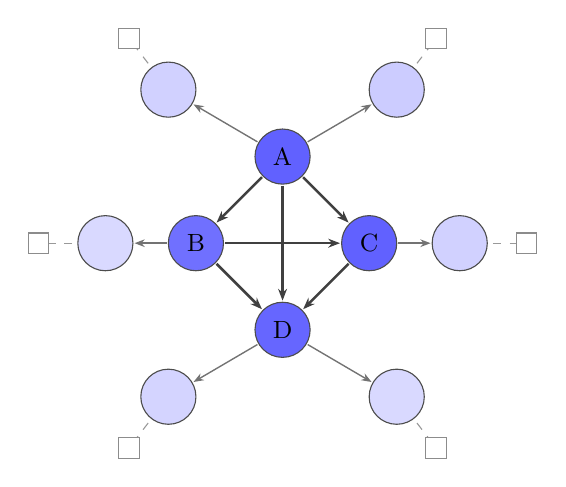
\begin{tikzpicture}
  \Positions \Edges
  \node[bel,fill=blue!62!white] at (A){A};
  \node[bel,fill=blue!56!white] at (B){B};
  \node[bel,fill=blue!62!white] at (C){C};
  \node[bel,fill=blue!60!white] at (D){D};
  \node[bel,fill=blue!18!white] at (b1){};
  \node[bel,fill=blue!20!white] at (b2){};
  \node[bel,fill=blue!15!white] at (b3){};
  \node[bel,fill=blue!18!white] at (b4){};
  \node[bel,fill=blue!17!white] at (b5){};
  \node[bel,fill=blue!15!white] at (b6){};
\end{tikzpicture}}
\par\vspace{4pt}
\resizebox{0.74\linewidth}{!}{%
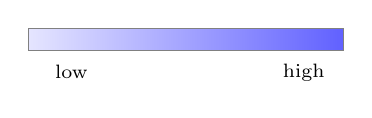
\begin{tikzpicture}
  \shade[left color=blue!10!white,right color=blue!62!white] (0,0) rectangle (4,0.28);
  \draw[black!50,line width=0.3pt] (0,0) rectangle (4,0.28);
  \node[font=\scriptsize] at (0.55,-0.28){low}; \node[font=\scriptsize] at (3.5,-0.28){high};
\end{tikzpicture}}
\caption{Revision cost $\kappa_i$ (conservatism)}
\label{sub:cost}
\end{subfigure}
\hfill
\begin{subfigure}{0.49\textwidth}\centering
\resizebox{0.92\linewidth}{!}{%
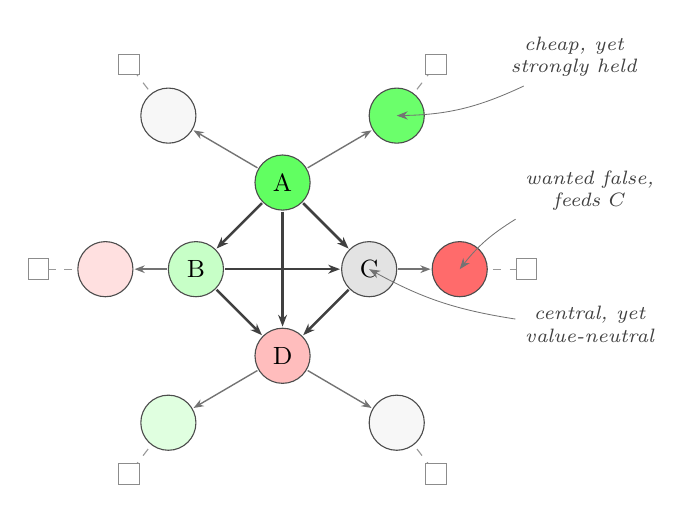
\begin{tikzpicture}
  \Positions \Edges
  \node[bel,fill=green!62!white] at (A){A};
  \node[bel,fill=green!22!white] at (B){B};
  \node[bel,fill=gray!22!white]  at (C){C};
  \node[bel,fill=red!26!white]   at (D){D};
  \node[bel,fill=gray!6!white]   at (b1){};
  \node[bel,fill=green!58!white] at (b2){};
  \node[bel,fill=red!12!white]   at (b3){};
  \node[bel,fill=red!58!white]   at (b4){};
  \node[bel,fill=green!12!white] at (b5){};
  \node[bel,fill=gray!6!white]   at (b6){};
  \node[anno] (an2) at (3.7,2.7){cheap, yet\\strongly held};
  \draw[annoarrow] (an2) to[bend left=12] (b2);
  \node[anno] (anC) at (3.9,-0.7){central, yet\\value-neutral};
  \draw[annoarrow] (anC) to[bend left=10] (C);
  \node[anno] (an4) at (3.9,1.0){wanted false,\\feeds $C$};
  \draw[annoarrow] (an4) to[bend right=10] (b4);
\end{tikzpicture}}
\par\vspace{4pt}
\resizebox{0.88\linewidth}{!}{%
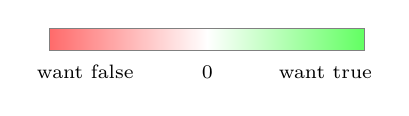
\begin{tikzpicture}
  \shade[left color=red!58!white,right color=white] (0,0) rectangle (2,0.28);
  \shade[left color=white,right color=green!62!white] (2,0) rectangle (4,0.28);
  \draw[black!50,line width=0.3pt] (0,0) rectangle (4,0.28);
  \node[font=\scriptsize] at (0.45,-0.28){want false}; \node[font=\scriptsize] at (2,-0.28){0};
  \node[font=\scriptsize] at (3.5,-0.28){want true};
\end{tikzpicture}}
\caption{Intrinsic utility $u_i$ (conviction)}
\label{sub:util}
\end{subfigure}
\caption{Two fields on one paradigm (schematic). Both panels carry the \emph{same} network---a densely
coupled core $\{A,B,C,D\}$ and a sparse belt $\{b_1,\dots,b_6\}$ in contact with observation.
\subref{sub:cost}~Revision cost is the carry-over of mind-change, $\kappa=\Top\bone$
(Eq.~\ref{eq:kappa}): a node's cost is the precision-weighted mass of its descendants, a clean radial
gradient monotone in centrality. \subref{sub:util}~Intrinsic utility is signed---beliefs one wants
true (green), wants false (red), or is neutral toward (white)---and the conviction field
$U=\Top u$ does not align with $\kappa$: $C$ is central yet value-neutral; $b_2$ is cheap yet strongly
held; $b_4$, which feeds $C$, is a conclusion the community wants false. The two fields are
$\Top\bone$ and $\Top u$, the same operator on two sources, and they are independent vectors.}
\label{fig:twofields}
\end{figure}

\subsection{Motivated revision and the lock-in parameter}
\label{sec:revision}

The bounded agent revises its belief $q(x)$ over the whole network by trading fidelity to the honest
posterior against the value of where the commitments land,
\begin{equation}
\mathcal{F}[q]\;=\;\KL{q(x)}{p(x\mid o,G)}\;-\;\lambda\,\Eq{q}{U^{\!\top}\!x},
\qquad\Longrightarrow\qquad
q_\lambda(x)\;\propto\;p(x\mid o,G)\,e^{\lambda\,U^{\!\top}\!x},
\label{eq:tilted}
\end{equation}
with $\lambda$ a single temperature governing how far value may bend the evidence. The operation
itself is classical---an exponential tilt of the posterior, the form KL-regularized utility
maximization always yields \citep{todorov2009,ortega2013}; what is ours is the source of the tilt, a
conviction field propagated through the paradigm's own operator. In the linear-Gaussian regime the
tilt is a pure mean shift, displacing the commitments by $\lambda\Sigma U$ and leaving the
covariance untouched (Appendix~\ref{app:operator}). What opposes the displacement is
evidence, also through the mean: a disconfirming channel $k$ with sensory precision $\rho_k$ and
read-out $H_k$ pulls the mean back with gain $\propto\rho_k\,H_k\Sigma U$. As conviction drives a
disconfirming channel toward $\rho_k\to0$ that gain vanishes: the channel can no longer move the
mean, and the value-displaced commitment stands unrefuted. The fraction of disconfirming sensory
precision so silenced,
\begin{equation}
\gamma\;=\;\frac{\sum_{k\in\mathrm{dis}}\rho_k\,\mathbb{1}[\,\rho_k\ \text{gated by the core}\,]}
{\sum_{k\in\mathrm{dis}}\rho_k},
\label{eq:gamma}
\end{equation}
is the \emph{lock-in parameter}. In the experiments nothing is silenced by hand: the more a
channel's reports threaten what the agent values, the less the agent listens. Concretely, each
round channel $k$ carries weight $w_k=\exp(-g\,|U\!\cdot\!H_k|)$, where $U\!\cdot\!H_k$ measures
how directly the channel bears on valued commitments and $g$ sets how strongly caring becomes
not-listening.

Note what this mechanism \emph{is}: a representation of which conclusions an agent values,
expressed as a displacement of where its beliefs come to rest---and, under forgetting, a
displacement that saturates (\S\ref{sec:temporal}) while evidence keeps arriving. A bias, not a
resistance. The results will make that distinction load-bearing.

\subsection{Structure learning: reduction and expansion}
\label{sec:structurelearning}

Structure learning revises $G$ itself---the first requirement of \S\ref{sec:hidden}, that
structure be the \emph{object} of inference, now discharged by two asymmetric operations
\citep{friston2017curiosity,smith2020structure}. The asymmetry is the formal counterpart of normal
versus revolutionary science.

\emph{Reduction} is the exact half. Each edge is parameterized by a prior precision $\alpha_e$
($\alpha_e\to\infty$ pins the edge's parameter to zero; $\alpha_e\to0$ frees it), the
automatic-relevance-determination parameterization of sparse Bayesian learning
\citep{mackay1992,tipping2001}. Bayesian model reduction \citep{friston2011,friston2018bmr} scores any
pruning in closed form from the already-inverted posterior,
\begin{equation}
\frac{p(o\mid\tilde M)}{p(o\mid M)}=\Eq{p(\theta\mid o)}{\frac{\tilde p(\theta)}{p(\theta)}},
\label{eq:bmr}
\end{equation}
the Savage--Dickey ratio in general form: one inversion scores every candidate reduced structure
without re-touching the data.

\emph{Expansion} reaches what reduction cannot: a commitment no one has represented. Following
\citet{friston2017curiosity}, the agent entertains a new node by wiring it tentatively to existing
nodes with free priors ($\alpha_e\to0$) and letting reduction prune the proposal back to the couplings
the data support. Expansion is not closed-form---a new node may enlarge the
likelihood's support and requires a real inversion---and this cost asymmetry is why a field
reorganizes its periphery continually and its centre only rarely. The agent does not plan \emph{when}
to expand: candidates arrive at a Poisson rate, and an arrival is kept only if the model log Bayes
factor favours the wired-in node (Appendix~\ref{app:crisis-discovery}). It must be a rate,
because one cannot plan toward a dimension one has not yet conceived---Stanford's problem of
unconceived alternatives \citep{stanford2006}, to which we return. The rate itself, however, is
not condemned to be a constant: like every precision in active inference it admits treatment as a
\emph{belief}---here, the agent's belief that its own model class is incomplete---and
Appendix~\ref{app:closing} gives it that treatment, with the constant rate retained as the agnostic
baseline every comparison is run against.

\subsection{Forgetting}
\label{sec:temporal}

The introduction asked how a community loses information it once held; forgetting is the model's
answer, and it is load-bearing rather than cosmetic. Read once from fixed precisions,
$\kappa=\Top\bone$ can only grow as learning adds edges: a paradigm
with no forgetting is a ratchet, and lock-in under it is automatic rather than earned. We import the
standard remedy unmodified: accumulated precision relaxes toward the prior between updates,
$\Pi\leftarrow\Pi_0+\omega(\Pi-\Pi_0)$ with forgetting factor $\omega\in(0,1]$
\citep{friston2017process,smith2022tutorial}, so a deposit $k$ steps old carries weight $\omega^k$.
The factor is the agent's prior on the world's structural drift---one forgets at the rate one believes
the structure is moving \citep{mathys2011}. The operator inherits the time index,
$\Top_t=(I-A_t)^{-1}$, and a once-central node whose couplings go unreinforced relaxes back toward
cheapness. With forgetting, the value tilt saturates at $\lambda U/(1-\omega)$ and competes with the
also-saturated per-step evidence, so conviction holds only above a threshold: an entrenched bloc
re-tracks a moving truth at low $\lambda$ and stays locked at high---motivated persistence turned
from a posited bias into a threshold conviction must clear.

\subsection{Conflict, and the reliability an agent infers from it}
\label{sec:reliability}

Everything so far is a default, and the defaults have a known pathology: they cannot represent
\emph{conflict}. Two classical theorems, one per level of the model, pin it down. \emph{Pooling
is a contraction}: precision-weighted averaging on a connected trust graph is DeGroot dynamics in
information form \citep{degroot1974}, and because its weights never depend on the \emph{content}
of what is pooled, the spread of beliefs contracts geometrically toward consensus---disagreement
can only decay, never regenerate, so a persistent school of thought is impossible by construction
\citep{catal2024}. \emph{Gaussian conflict resolves by compromise}: within an agent, a posterior
built from light-tailed sources responds to contradiction between them with a confident
average---it can never reject a conflicting source, however extreme
\citep{dawid1973,ohagan1979}---and its precision \emph{grows} while doing so \citep{ohagan2012}:
contradiction makes a Gaussian agent more certain, never less. There is no slot in $(\Pi,h)$ for
being torn. Together the theorems make the default community a \emph{null regime}: the simplest
faithful model of a believing, communicating population, in which crisis, schism, and schools
provably cannot arise---only smooth, cumulative refinement of the frame everyone already shares.

The conflict-resolution literature's canonical repair \citep{ohagan2012} is to stop treating each
source's precision as a constant and infer it. We carry the repair as a scale mixture: each
channel's noise precision is a latent with its own prior, and its posterior expectation, given
the standardized one-step surprise $z_k^2$ (the squared residual of observation $k$ against the
agent's own prediction, in units of its predictive variance), is the classic Student-$t$ weight
\begin{equation}
\lambda_k \;=\; \frac{\nu+1}{\nu+z_k^2},
\label{eq:lambda}
\end{equation}
applied multiplicatively to the channel's evidence deposit. The rule is one sentence: \emph{trust
what does not keep surprising you}. A channel reporting on-prediction ($z^2\!\sim\!1$) keeps full
weight; a gross outlier is discounted as $\nu/z^2$---inferred unreliable rather than averaged
in---and the single dial $\nu$ sets how quickly surprise becomes doubt ($\nu\to\infty$ recovers
the Gaussian defaults exactly).

The same functional gates trust \emph{between} agents: $\gamma_{ij}=(\nu_s+1)/(\nu_s+z_{ij}^2)$,
with $z_{ij}^2$ now the calibrated disagreement between $i$'s and $j$'s posteriors, summed over
the commitments both measure---summed, not averaged, because a \emph{localized} disagreement must
be able to sever trust; a mean over many agreed-upon nodes would dilute any heresy below the
gate's notice. The fusion weights of the pooling step are multiplied by $\gamma$, so an agent
keeps averaging with neighbours it can predict and quietly stops listening to those it cannot.
And because $z^2$ is just a calibrated gap, the gate can be pointed at different things: at
\emph{opinions} (the posterior means above), or at \emph{wiring}---the contested coupling entries
of $\Pi$ itself, a scale-invariant read of how differently two agents structure the world
(Appendix~\ref{app:reliability}). Where it is pointed will turn out to matter
(\S\ref{sec:res-pluralism}).

Note what the gate is not. It adds no objective, no memory, and no new fixed point: $\lambda$ and
$\gamma$ are instantaneous functions of the current surprise, every weight stays strictly
positive, and the contraction theorem still owns the long run---consensus remains the only place
the dynamics can rest. Whatever the gate buys, it can only buy as \emph{time}. The results
measure how much.

% ======================================================================
\subsection{The population, and the simulation at a glance}
\label{sec:model}
% ======================================================================

The third requirement of \S\ref{sec:hidden}---communication---enters here, in its default form.
A population of $N$ agents inhabits a shared hidden world, each carrying its own paradigm network
with its own coupling precisions, conviction field $U=\Top u$, and derived conservatism
$\kappa=\Top\bone$. Agents are coupled on a trust graph: communities are blocks of a stochastic block
model, with dense intra-community edges and an inter-community coupling weight (\emph{inter}) that we
sweep from total isolation to dense contact. Beliefs and accumulated precisions are fused across
trust edges in information form---a precision-weighted pooling of posteriors in which an agent's own
evidence and its neighbours' carry weight in proportion to trust, the information-form counterpart
of trust-weighted averaging in opinion dynamics \citep{degroot1974,acemoglu2011}---and what is not
standard is that structural edits spread the same way: an agent whose neighbour has awakened a new node receives the proposal and scores it
against its own model by Eq.~\eqref{eq:bmr}. Figure~\ref{fig:population} draws the picture: what
travels on the trust graph is not a number but a piece of structure, evaluated against wiring the
sender does not see.

\begin{figure}[h!]
\centering
\resizebox{0.92\linewidth}{!}{%
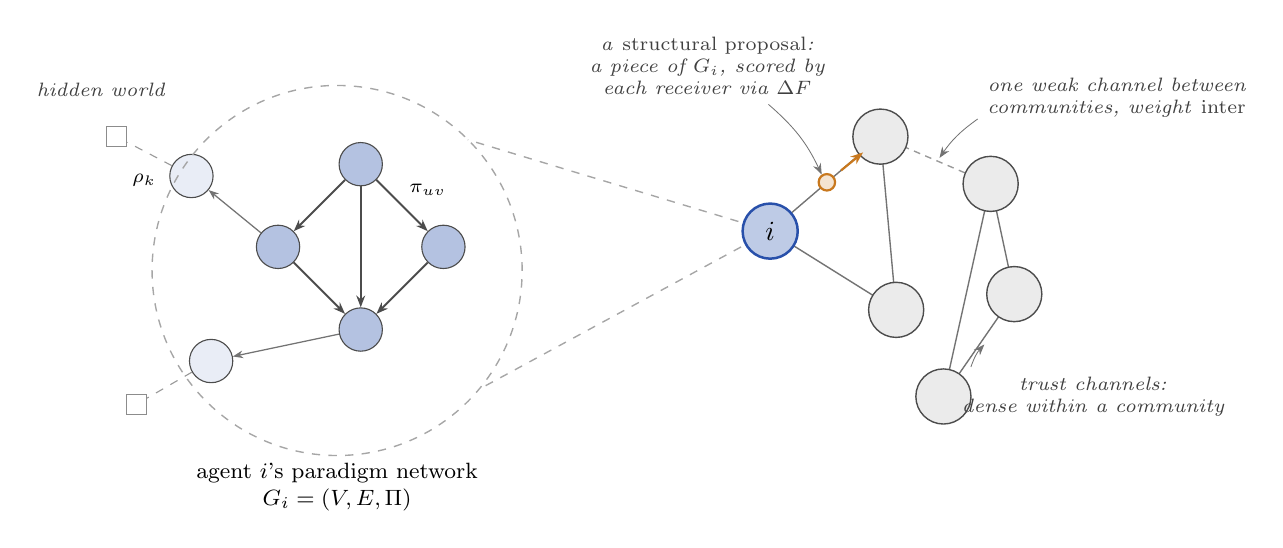
\begin{tikzpicture}[
  n/.style={circle,draw=black!70,line width=0.4pt,fill=costc!35,minimum size=5.5mm,inner sep=0pt},
  nb/.style={circle,draw=black!70,line width=0.4pt,fill=costc!10,minimum size=5.5mm,inner sep=0pt},
  ag/.style={circle,draw=black!70,line width=0.5pt,fill=black!8,minimum size=7mm,inner sep=0pt},
  dep/.style={-{Stealth[length=1.5mm]},line width=0.7pt,black!70},
  depb/.style={-{Stealth[length=1.3mm]},line width=0.45pt,black!55}]
  % ---- left: agent i's paradigm network, magnified ----
  \node[n] (A) at (0,1.05) {};
  \node[n] (B) at (-1.05,0) {};
  \node[n] (C) at (1.05,0) {};
  \node[n] (D) at (0,-1.05) {};
  \node[nb] (b1) at (-2.15,0.9) {};
  \node[nb] (b2) at (-1.9,-1.45) {};
  \draw[dep] (A)--(B); \draw[dep] (A)--(C); \draw[dep] (A)--(D);
  \draw[dep] (B)--(D); \draw[dep] (C)--(D);
  \draw[depb] (B)--(b1); \draw[depb] (D)--(b2);
  \node[obs] (o1) at (-3.1,1.4) {};
  \node[obs] (o2) at (-2.85,-2.0) {};
  \draw[sens] (b1)--(o1); \draw[sens] (b2)--(o2);
  \node[font=\scriptsize] at (0.85,0.72) {$\pi_{uv}$};
  \node[font=\scriptsize] at (-2.75,0.85) {$\rho_k$};
  \node[anno] at (-3.3,2.0) {hidden world};
  % the agent's boundary, pierced by its sensory channels
  \draw[black!35,dashed,line width=0.5pt] (-0.3,-0.3) circle (2.35);
  \node[font=\footnotesize,align=center] at (-0.3,-3.05)
    {agent $i$'s paradigm network\\$G_i=(V,E,\Pi)$};
  % ---- magnifier lines to one agent of the trust graph ----
  \draw[black!35,dashed,line width=0.5pt] (5.2,0.2) -- (1.36,1.36);
  \draw[black!35,dashed,line width=0.5pt] (5.2,0.2) -- (1.5,-1.81);
  % ---- right: the trust graph, two communities ----
  \draw[belt] (5.2,0.2)--(6.6,1.4); \draw[belt] (5.2,0.2)--(6.8,-0.8);
  \draw[belt] (6.6,1.4)--(6.8,-0.8);
  \draw[belt] (8.0,0.8)--(8.3,-0.6); \draw[belt] (8.3,-0.6)--(7.4,-1.9);
  \draw[belt] (8.0,0.8)--(7.4,-1.9);
  % the single weak channel between communities
  \draw[line width=0.5pt,black!40,dash pattern=on 2.4pt off 2pt] (6.6,1.4)--(8.0,0.8);
  \node[ag,fill=costc!30,draw=costc,line width=0.9pt] (ai) at (5.2,0.2) {$i$};
  \node[ag] (a2) at (6.6,1.4) {};
  \node[ag] (a3) at (8.0,0.8) {};
  \node[ag] (a4) at (6.8,-0.8) {};
  \node[ag] (a5) at (8.3,-0.6) {};
  \node[ag] (a6) at (7.4,-1.9) {};
  \node[anno] (anInter) at (9.6,1.9) {one weak channel between\\communities, weight \emph{inter}};
  \draw[annoarrow] (anInter) to[bend right=10] (7.35,1.13);
  \node[anno] (anTrust) at (9.3,-1.9) {trust channels:\\dense within a community};
  \draw[annoarrow] (anTrust) to[bend left=12] (7.92,-1.24);
  % ---- the object being passed: a structural proposal ----
  \node[circle,draw=newc,line width=0.8pt,fill=newc!20,inner sep=2.1pt] (prop) at (5.92,0.82) {};
  \draw[-{Stealth[length=1.6mm]},newc,line width=0.8pt] (6.1,0.97) -- (6.38,1.2);
  \node[anno] (anProp) at (4.4,2.3) {a \emph{structural proposal}:\\a piece of $G_i$, scored by\\each receiver via $\Delta F$};
  \draw[annoarrow] (anProp) to[bend left=12] (prop);
\end{tikzpicture}}
\caption{The population model. Right: the community is a trust graph, every circle an agent. Left,
magnified: each agent privately holds a paradigm network $G_i=(V,E,\Pi)$---commitments coupled by
precisions $\pi_{uv}$, a belt reading the hidden world through sensory channels of precision
$\rho_k$---from which its conservatism $\kappa=\Top\bone$ and conviction $U=\Top u$ are derived. What
passes along trust channels (amber) is a \emph{structural proposal}: a piece of paradigm, e.g.\ a
newly awakened node, which each receiver scores against its own network by $\Delta F$
(Eq.~\ref{eq:bmr}); posteriors fuse precision-weighted along the same channels. The trust graph is
fixed at the start (a stochastic block model): channels are dense and strong inside a community, and
a single weak weight \emph{inter}---the main dial of \S\ref{sec:results}---connects communities, so
what reaches an agent from outside is its neighbours' evidence and proposals, scaled by trust.}
\label{fig:population}
\end{figure}

Concretely, the experiments of \S\ref{sec:results} instantiate the phlogiston world: a hub-structured
paradigm net in which a single core commitment (phlogiston) is load-bearing for combustion,
calcination and respiration; at a fixed step $t_{\mathrm{shift}}$ the world's regime flips (the calx
is heavier---the gravimetric anomaly), and the truth thereafter contains a dimension (oxygen) that is
\emph{not in any agent's network}. One round of the simulation, for every agent:

\begin{enumerate}\itemsep1pt
\item \textbf{Observe.} The world emits observations at the belt; channel weights on disconfirming
rows are set endogenously by the conviction gate, $w_k=\exp(-g\,|U\!\cdot\!H_k|)$
(\S\ref{sec:revision}), scaled by the agent's gate strength $s$. With the reliability gate on,
each deposit is further weighted by the channel's inferred reliability $\lambda_k$
(Eq.~\ref{eq:lambda}).
\item \textbf{Infer.} The agent updates its (value-tilted, Eq.~\ref{eq:tilted}) posterior over $x$ by
exact linear-Gaussian inference and accumulates precision.
\item \textbf{Crisis check (reduction).} Each candidate prune is scored on the move ledger: the
closed-form prune evidence $\Delta F$ (Eq.~\ref{eq:bmr}) plus $\lambda_i$ times the equally
closed-form conviction-value change of the prune,
$\Delta U = U^{\!\top}\!(\mu_{\mathrm{reduced}}-\mu)$, read from the reduced posterior the
Savage--Dickey identity already exhibits. Both protective belt edges scoring
$\Delta F + \lambda_i\,\Delta U > 0$ is a \emph{crisis}, and the agent applies the reduction---the
hub is released (Appendix~\ref{app:crisis-discovery}).
\item \textbf{Discovery check (expansion).} After reduction, the residual the old paradigm absorbed
becomes visible as a coherent pattern in prediction error; when a Poisson proposal arrives (rate
$r$), its \emph{direction} is read from that pattern's leading eigenvector, and the wake is
accepted iff the model log Bayes factor is positive---the data must hold the new node
(\S\ref{sec:structurelearning}, Appendix~\ref{app:crisis-discovery}). The rate is constant in
the baseline; Appendix~\ref{app:closing} makes it a posterior and a social process, and replaces the
one-shot accept with an audited wake-then-prune cycle.
\item \textbf{Fuse.} Posteriors and structural edits are pooled across the trust graph, weighted by
the intra/inter coupling---and, with the social gate on, by the inferred trust $\gamma_{ij}$
(\S\ref{sec:reliability}). Whether agents pool over \emph{all} dimensions or only over those they
jointly represent is a protocol choice with consequences (Appendix~\ref{app:null}).
\item \textbf{Forget.} Accumulated precision decays by $\omega$ (\S\ref{sec:temporal}).
\end{enumerate}

Crisis, revolution and discovery are thus not stipulated events but threshold crossings of the
model's own evidence; Appendix~\ref{app:crisis-discovery} derives both checks from the single
tilted objective and lists explicitly what remains a modelling commitment.
Table~\ref{tab:dials} (Appendix~\ref{app:null}) lists the dials swept; everything else is held
fixed, and all code is seeded and ships its own null and positive controls.

One thing deserves emphasis before the results: every ingredient above is its field's default.
The belief model is the workhorse of Kalman filtering and structural equations; the value
mechanism is the standard formalization of motivated reasoning; the fusion step is classical
opinion pooling in information form; expansion and reduction are textbook Bayesian model
comparison. Nothing exotic has been smuggled in. The sweep that follows tests what these
defaults can do \emph{together}.

% ======================================================================
\section{Results}
\label{sec:results}
% ======================================================================

All results are from the population of \S\ref{sec:model} run on the phlogiston world---normal
science, the gravimetric anomaly, crisis, reduction, discovery of oxygen, new normal, every phase
a threshold crossing of the agents' own evidence, none stipulated. The nets are hand-wired to
expose the geometry, not fitted to data: nothing here is evidence about chemistry, only about how
a structured, bounded, valued mind changes. We first state what the default community does, then
switch on the gate of \S\ref{sec:reliability}---first within agents, then between them---and
follow the cycle through crisis, schism, and rehabilitation.

\subsection{The null regime, measured}
\label{sec:res-null}

With every reliability fixed, the sweep (2{,}488 runs; figures and the full mechanism table in
Appendix~\ref{app:null}) confirms the theorems and locates their boundary. Within an agent,
conviction tilts where beliefs settle, never when they yield: value buys a biased resting place,
not a delayed reckoning \citep{hyland2025}, and its one causal route to lock-in runs through
gating one's own disconfirming channels. At population scale that protection loses to the
faintest connection: at \emph{inter}$=0.005$---trust toward outsiders two hundred times weaker
than trust within the community---$92\%$ of the dogmatic community converts, however dogmatic,
because fusion shares \emph{evidence}, not conclusions: an agent can silence its own instruments,
not its neighbours' (Fig.~\ref{fig:res-lockin}). Between agents, pooling kills the lone
discoverer---a concept woken by one agent at a time is averaged away by peers whose priors read
\emph{has no such variable} as \emph{certainly zero}---and every mechanism we layered on the
baseline (adequacy-driven exploration, social excitation, audited curiosity, value accretion)
either re-times the passage to consensus or synchronizes the population for it; none lets two
connected communities holding the same data remain in disagreement
(Table~\ref{tab:escapes}). The null regime is normal science, and nothing in it can do anything
else.

\subsection{Within an agent: conflict becomes crisis, and points to its own cause}
\label{sec:res-conflict}

The smallest possible setting already shows everything the channel gate changes. One agent holds
a three-commitment chain $A\!\to\!B\!\to\!C$; at step $30$ channel $A$ turns persistently
contradictory---the world keeps reporting a value the rest of the agent's network cannot
reconcile. The Gaussian baseline does what the theorem says it must: it settles confidently
between the channel's report and what its own couplings imply ($\mu_A=-2.0$, a configuration
neither source supports), its variance falling monotonically throughout---the conflict leaves
\emph{no trace} in the belief state. The gated agent instead infers the channel unreliable
($\lambda_A$ falls to $0.16$), and its uncertainty does something no light-tailed posterior can:
it \emph{rises} while evidence accumulates, peaking eight steps after the conflict begins before
recovering (Fig.~\ref{fig:res-variance})---crisis as suspended confidence, rendered as a
posterior. The conflict also becomes \emph{localizable}: edge strain
(Appendix~\ref{app:reliability}), a cheap per-step read of how hard each edge fights the agent's
own data, ranks the violated coupling above the innocent one at every step, so the Bayes-factor
verdict of Eq.~\eqref{eq:bmr} need only be paid where the strain points---targeted, rather than
scanned, model reduction.

\begin{figure}[h!]
\centering
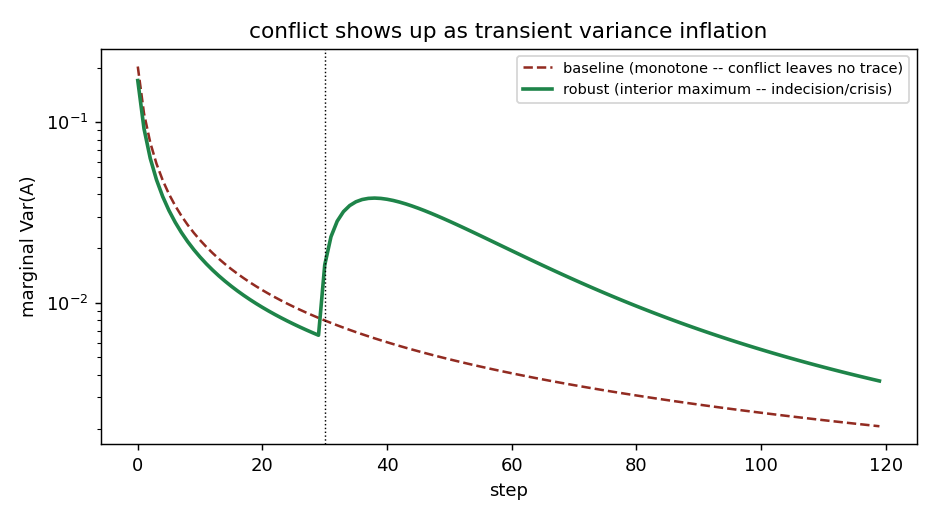
\includegraphics[width=0.62\linewidth]{fig_abc_variance.png}
\caption{Conflict as suspended confidence. A channel turns contradictory at step 30 (dotted
line). The Gaussian baseline (dashed) grows monotonically more certain---the confident
compromise; the gated agent's marginal variance (solid) shows an interior maximum: doubt rises
while data accumulate, then resolves as the discounted channel is reorganized around. There is
now a slot in the belief state for being torn.}
\label{fig:res-variance}
\end{figure}

\subsection{The community: denial, delay, rehabilitation}
\label{sec:res-crisis}

Run the same gate in the full population through the regime flip
(Fig.~\ref{fig:res-crisistrace}). At the flip, the anomalous channels become surprising, so the
community infers \emph{them} unreliable first: their mean inferred reliability collapses from
above $0.85$ to $0.17$ while the unaffected channels stay fully trusted throughout---selective
denial; the instruments are doubted before the theory, which is how the chemists actually
received the gravimetric anomaly. The discounted evidence still trickles in, so belief drifts;
as it drifts, the anomaly grows less surprising, the gate \emph{rehabilitates} the channels it
condemned (final $\bar\lambda=1.27$), and conversion completes---$4.3\times$ later than the
fixed-precision slide, on the same evidence. The shape is worth stating precisely, because the
gate's feedback here is \emph{self-stabilizing} (each agent's surprise falls as its own belief
moves): the channel gate \emph{throttles} the conversion---a stretched, decelerating slide, not
a stall that breaks---and harsher gates only stretch it further. The sudden half of the Kuhnian
shape is real but lives one level up, in the trust gate, whose feedback is \emph{collective}:
there, a leak shrinks the inter-camp gap, which reopens the gate, which accelerates the
leak---and the merge arrives late and fast (\S\ref{sec:res-schools}).

\begin{figure}[h!]
\centering
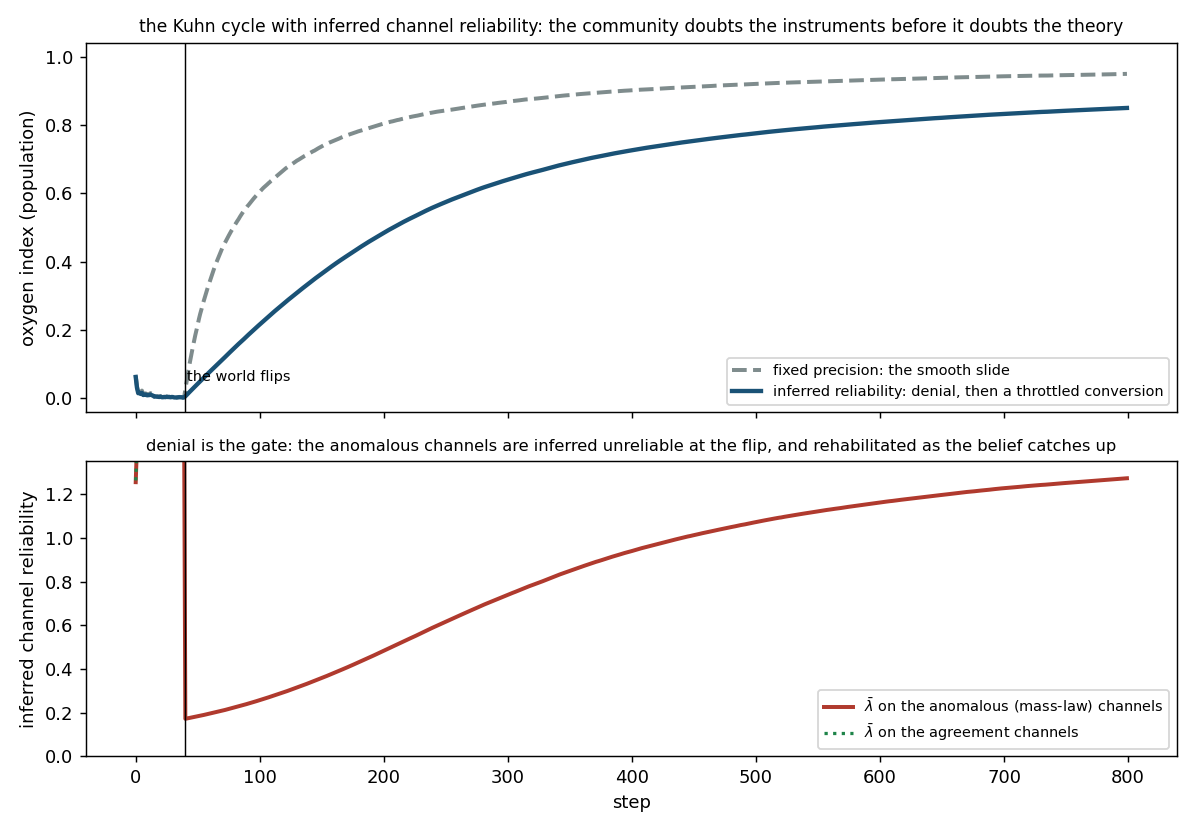
\includegraphics[width=0.74\linewidth]{fig_crisis_trace.png}
\caption{The Kuhn cycle with inferred channel reliability ($N=20$, world flips at the vertical
line). \emph{Top:} population conversion. Fixed precision (dashed) slides from the flip; the
gated community (solid) converts on the same evidence at a fraction of the rate---denial
throttles, it does not break. \emph{Bottom:} the mechanism. Mean inferred reliability
$\bar\lambda$ on the anomalous channels collapses at the flip---denial---while the agreement
channels stay trusted; as belief catches up, the channels the community condemned are
rehabilitated. Doubt the instruments first, the theory later.}
\label{fig:res-crisistrace}
\end{figure}

\subsection{Between communities: distrust buys time; confidence buys a schism}
\label{sec:res-schools}

Point the gate at peers and the contraction theorem's grip loosens---into timescales, exactly as
\S\ref{sec:reliability} promised. The cleanest setting first: two opposed camps on a
\emph{complete} graph, no topology to hide behind. Uniform fusion collapses their disagreement
to $0.1\%$ of its initial value within a couple of steps; with the gate on, each camp infers the
other not worth listening to (cross-camp trust settles at $0.8\%$ of within-camp), and $48\%$ of
the initial separation survives the whole horizon. Stable schools, on a connected graph, holding
shared data---the configuration the fixed-trust regime forbids---are now \emph{attainable}, as
metastable states rather than fixed points.

What decides whether they are \emph{attained} is confidence. Sweeping how much evidence the two
camps accumulated before contact (Fig.~\ref{fig:res-schism}) yields a sharp threshold: below it
the gated population merges exactly like the fixed-trust control ($<1\%$ of disagreement
survives); above it most of the disagreement outlives the run ($17\%/48\%/76\%$ as confidence
doubles past the threshold), because the gate reads the calibrated gap
$z^2\sim\text{gap}^2\times\text{precision}$: camps that merely believed differently with more
confidence are more mutually surprising. Precision being the integral of exposure time,
confidence at contact is what incubation \emph{buys}: incommensurability is not a property of
two ideas but of two histories, and it has a clock.

\begin{figure}[h!]
\centering
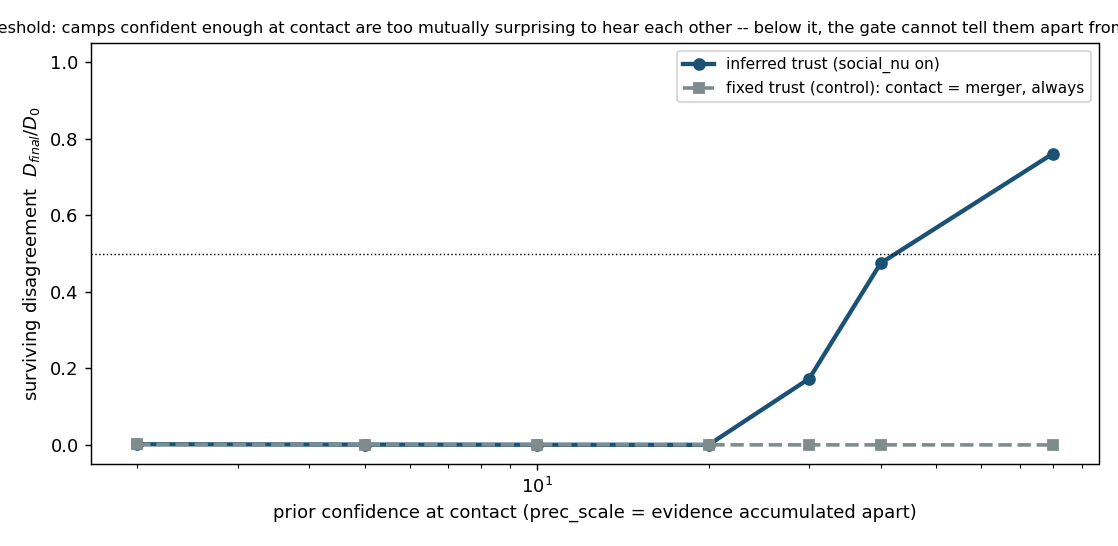
\includegraphics[width=0.6\linewidth]{fig_schism_threshold.png}
\caption{The schism threshold (two opposed camps, full contact, complete graph). $x$-axis: prior
confidence at contact (evidence accumulated apart); $y$-axis: fraction of the initial
disagreement surviving the horizon. Under fixed trust (squares) contact is merger at every
confidence ($\le0.2\%$ survives). Under inferred trust (circles) there is a sharp interior
threshold: below it the gate cannot tell the camps apart from the control; above it the camps
sever trust and most of the disagreement survives. Confidence is the clock of
incommensurability.}
\label{fig:res-schism}
\end{figure}

The full Kuhn cycle puts both halves together (Fig.~\ref{fig:res-rehab}). Re-running the null
regime's lock-in boundary with inferred trust, the dogmatic community now \emph{builds its own
wall}: as the open community converts, cross-community trust collapses below $1\%$ of
within-community trust---self-organized isolation, nothing silenced by hand. But mid-cycle
dogmatists have not yet accumulated a schism's worth of confidence, and the gate is memoryless:
the evidence that leaks through the still-positive weights moves the laggards, the gap shrinks,
the gate \emph{reopens}, and the merge cascades---genuinely late and fast, with the laggards'
conversion rate peaking at step $126$ of $180$, the slow-then-sudden shape the self-stabilizing
channel gate of \S\ref{sec:res-crisis} cannot produce. Where fixed trust converts the dogmatic
community at \emph{inter}$=0.005$ with $t_{1/2}=78$ steps, the gated community needs
$146$--$170$ and is still incomplete at the horizon ($0.54$--$0.73$ converted vs.\ $0.92$); and
the trust the gate severed is \emph{rehabilitated} by the merge it failed to prevent (final
cross-community trust above $90\%$ of within). Distrust, inferred, has the arc fixed trust
cannot draw: distrust $\to$ plateau $\to$ rehabilitation $\to$ merge.

\begin{figure}[h!]
\centering
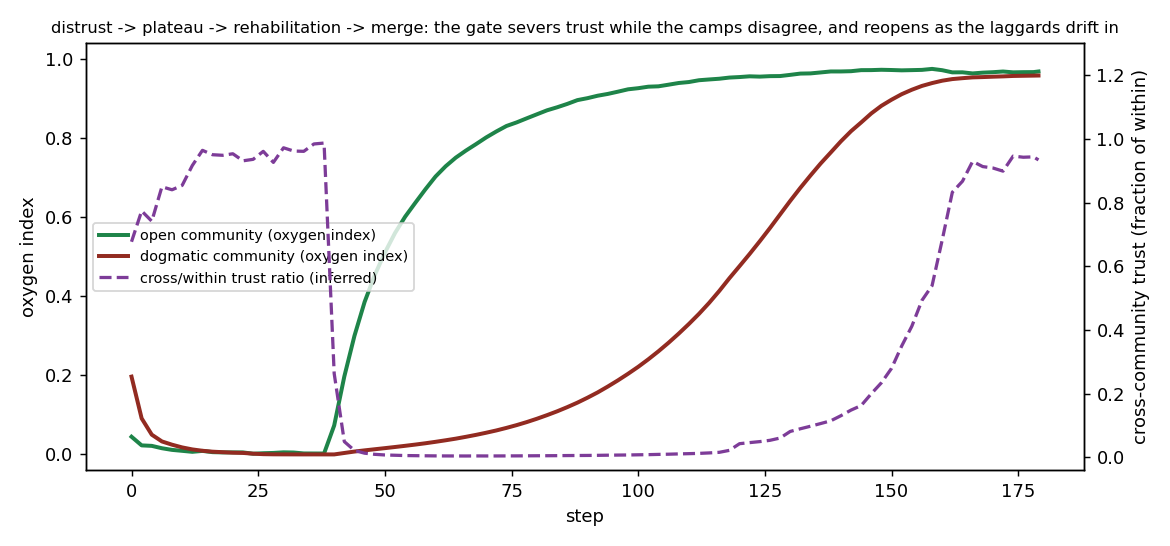
\includegraphics[width=0.76\linewidth]{fig_rehabilitation.png}
\caption{The rehabilitation arc (full Kuhn cycle, inferred trust, \emph{inter}$=0.05$). As the
open community converts (green) the camps diverge and inferred cross-community trust (dashed,
right axis) collapses to ${\sim}1\%$ of within-community trust: the gate severs the channel, and
the dogmatic community (red) plateaus at the old paradigm. The leak through the still-positive
weights moves the laggards; as they drift in, the gap shrinks, the gate reopens, and the merge
completes---restoring the trust whose absence it had inferred. Distrust buys time, not a wall.}
\label{fig:res-rehab}
\end{figure}

\subsection{Pluralism lives in the wiring---and only wiring-reading trust can keep it}
\label{sec:res-pluralism}

Everything above gates on \emph{opinions}: the posterior means. The last experiment asks what
happens when what divides two communities is not where their beliefs sit but how they are
\emph{wired}---the situation the introduction began with. In a world genuinely underdetermined
between two structures, two communities, attending differently because they value different
conclusions, learn the two different wirings. Connect them under fixed trust and averaging
dilutes both into one blurry compromise net ($10\%$ of the structural divergence survives).
Connect them under the \emph{opinion}-reading gate and exactly the same collapse occurs
($10.2\%$)---the gate never fires, because both camps fit the same blended data and so
\emph{agree in their means}: a trust that reads opinions is blind to a pluralism that lives in
wiring. Point the same Student-$t$ functional at the contested couplings of $\Pi$ instead
(\S\ref{sec:reliability}), and $94\%$ of the divergence survives full contact, across the whole
mixing sweep (Fig.~\ref{fig:res-wiring}). The collective, meanwhile, knows more than its members
only as a \emph{union}: averaging never creates an edge no member holds (measured synergy is
exactly zero), so the two-wiring knowledge exists in the population precisely as long as the
camps do.

\begin{figure}[h!]
\centering
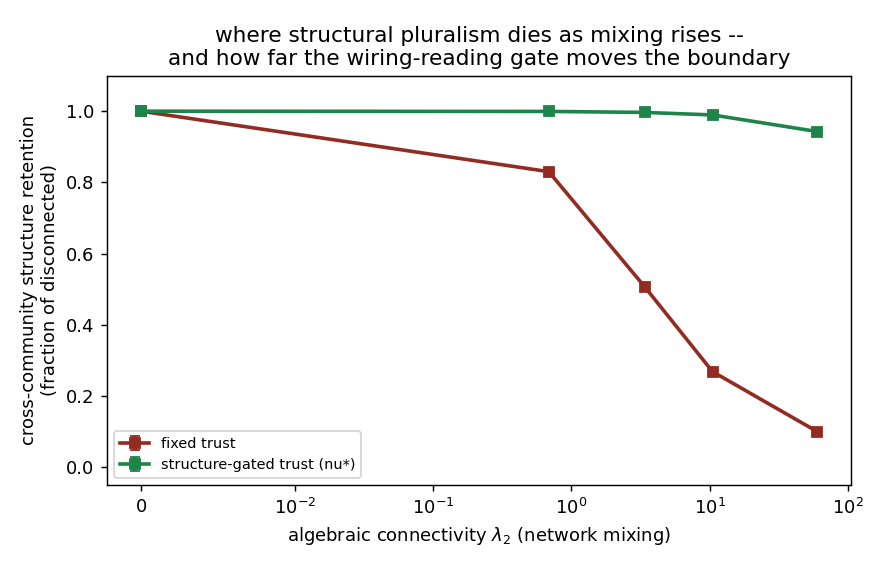
\includegraphics[width=0.6\linewidth]{fig_connectivity_boundary.png}
\caption{Where structural pluralism dies as mixing rises. $x$-axis: algebraic connectivity of
the contact graph; $y$-axis: surviving cross-community structure (fraction of the disconnected
benchmark). Fixed trust (red) dilutes both wirings toward one compromise net as mixing rises;
the wiring-reading gate (green) preserves the two learned structures at $94\%$ even under dense
contact. The opinion-reading gate (not shown) tracks the red curve: the camps agree in means,
so it never fires.}
\label{fig:res-wiring}
\end{figure}

One prediction this experiment \emph{refuted}, and the refutation is a scope condition worth
stating plainly. We expected a third camp, committed to a wiring the data do not support, to
fail to consolidate it. It consolidates it exactly as strongly as the supported camps do: in
linear-Gaussian Fisher learning the precision deposit never sees the observation's
\emph{value}---attention alone fabricates the coupling pattern, and the data's verdict on an
unsupported theory lives in the means, not in $|\Pi|$. Structure-as-precision-pattern, in this
model class, is attention-driven: the wiring gate can protect a pluralism, but it cannot tell a
supported school from a merely committed one. That discrimination belongs to the means---and to
the strain and reliability reads that live on them (\S\ref{sec:res-conflict}).

\paragraph{Controls.}
Every experiment ships its own null and positive controls: a world that never shifts produces
neither denial nor delay ($\lambda$ stays above $0.85$ on every channel); the fixed-trust arm
reproduces the null regime byte-identically (both gates default to off); low-confidence camps
merge indistinguishably from the control; and no acceptance bar is tuned anywhere---the wake's
sole accept test remains the model log Bayes factor (Appendix~\ref{app:crisis-discovery}).
Configurations, seeds, and the per-experiment headline numbers are tabulated in
Appendix~\ref{app:reliability}.

% ======================================================================
\section{Discussion}
\label{sec:discussion}
% ======================================================================

The model's relation to Kuhn can now be stated without allegory, in both directions. The default
community is the formalism's \emph{normal-science} limit: smooth, cumulative refinement within a
shared frame, with a hard core and protective belt that are derived rather than decreed
\citep{lakatos1970}, and provably nothing else. One inferred quantity---reliability, read off
surprise and applied alike to instruments and to peers---supplies the revolutionary remainder as
\emph{dynamics}: crisis as suspended confidence (the interior variance maximum of
\S\ref{sec:res-conflict}), denial as selective instrument-doubt that throttles conversion
(\S\ref{sec:res-crisis}), the late, fast merge of a reopening trust gate, incommensurability as
a confidence threshold with a clock, and schools, schisms, and rehabilitations as metastable
states of one trust functional (\S\ref{sec:res-schools}). None of these is stipulated; all of them are the Student-$t$ weight
of Eq.~\eqref{eq:lambda}, pointed at different parts of the agent's world.

The recurring price is the result we most want the reader to keep: \emph{everything the gate
buys, it buys as time}. The gate is memoryless, its weights stay positive, and consensus remains
the only fixed point---so dogma, denial, schism, and school are not different dynamics but the
same dynamics on slower clocks, and each protection ends by undoing itself (the trust the gate
severed is rehabilitated by the merge it delayed). This is the same shape forgetting gave
conviction in \S\ref{sec:temporal}: protection in this model class is always a race between
rates, never an absorbing state. Whether \emph{real} communities enjoy any protection stronger
than a timescale---or whether incommensurability was only ever patience running out---the model
converts from a metaphor into a measurable claim.

For communities of reasoning machines the statement is a design rule. Any aggregation step that
averages rather than gates inherits the null regime, whatever the sophistication of its members:
it will refine frames and never grow, hold, or split one. Gating restores open-endedness only if
it is pointed at the right level---a gate on opinions preserved nothing of a pluralism that
lived in wiring (\S\ref{sec:res-pluralism}). Open-endedness in a population of structure
learners is a property of the pooling protocol and of \emph{what the protocol reads}, to be
designed in; it is not an emergent grace of scale.

Two limits bound the claims, honestly. First, in this model class the precision-pattern is
attention-driven: data cannot veto an unsupported wiring (the refuted prediction of
\S\ref{sec:res-pluralism}), so the wiring gate protects pluralism without certifying it---the
world's verdict stays in the means. Second, everything revolutionary here passes through model
expansion over a fixed likelihood, while a genuinely new \emph{instrument} enlarges the
likelihood's own support; one cannot place a posterior over the unconceived
\citep{stanford2006}, only over whether one's model has missed something. What a community
controls is how hard it looks, what its pooling does to the member who finds it first---and now,
how long its distrust is allowed to last.

% ======================================================================
\begin{thebibliography}{99}

\bibitem[Albarracin et al.(2022)]{albarracin2022}
M.~Albarracin, D.~Demekas, M.~J.~D.~Ramstead, and C.~Heins.
Epistemic communities under active inference. \emph{Entropy}, 24(4):476, 2022.

\bibitem[\c{C}atal et al.(2024)]{catal2024}
O.~\c{C}atal, T.~Van~de~Maele, R.~J.~Pitliya, M.~Albarracin, C.~Pattisapu, and T.~Verbelen.
Belief sharing: a blessing or a curse. arXiv:2407.02465, 2024.

\bibitem[Dalege et al.(2016)]{dalege2016}
J.~Dalege, D.~Borsboom, F.~van Harreveld, H.~van den Berg, M.~Conner, and H.~L.~J.~van der Maas.
Toward a formalized account of attitudes: the Causal Attitude Network (CAN) model.
\emph{Psychological Review}, 123(1):2--22, 2016.

\bibitem[Dawid(1973)]{dawid1973}
A.~P.~Dawid.
Posterior expectations for large observations. \emph{Biometrika}, 60(3):664--667, 1973.

\bibitem[O'Hagan(1979)]{ohagan1979}
A.~O'Hagan.
On outlier rejection phenomena in Bayes inference.
\emph{Journal of the Royal Statistical Society, Series B}, 41(3):358--367, 1979.

\bibitem[O'Hagan and Pericchi(2012)]{ohagan2012}
A.~O'Hagan and L.~Pericchi.
Bayesian heavy-tailed models and conflict resolution: a review.
\emph{Brazilian Journal of Probability and Statistics}, 26(4):372--401, 2012.

\bibitem[Friedman et al.(2008)]{friedman2008glasso}
J.~Friedman, T.~Hastie, and R.~Tibshirani.
Sparse inverse covariance estimation with the graphical lasso.
\emph{Biostatistics}, 9(3):432--441, 2008.

\bibitem[Friston and Penny(2011)]{friston2011}
K.~J.~Friston and W.~Penny.
Post hoc Bayesian model selection. \emph{NeuroImage}, 56(4):2089--2099, 2011.

\bibitem[Friston et al.(2015)]{friston2015}
K.~Friston, F.~Rigoli, D.~Ognibene, C.~Mathys, T.~Fitzgerald, and G.~Pezzulo.
Active inference and epistemic value. \emph{Cognitive Neuroscience}, 6(4):187--214, 2015.

\bibitem[Friston et al.(2017)]{friston2017curiosity}
K.~J.~Friston, M.~Lin, C.~D.~Frith, G.~Pezzulo, J.~A.~Hobson, and S.~Ondobaka.
Active inference, curiosity and insight. \emph{Neural Computation}, 29(10):2633--2683, 2017.

\bibitem[Friston et al.(2018)]{friston2018bmr}
K.~J.~Friston, T.~Parr, and P.~Zeidman.
Bayesian model reduction. arXiv:1805.07092, 2018.

\bibitem[Hawkes(1971)]{hawkes1971}
A.~G.~Hawkes.
Spectra of some self-exciting and mutually exciting point processes.
\emph{Biometrika}, 58(1):83--90, 1971.

\bibitem[Hohwy(2016)]{hohwy2016}
J.~Hohwy.
The self-evidencing brain. \emph{No\^us}, 50(2):259--285, 2016.

\bibitem[Hughes et al.(2024)]{hughes2024}
E.~Hughes, M.~Dennis, J.~Parker-Holder, F.~Behbahani, A.~Mavalankar, Y.~Shi, T.~Schaul, and
T.~Rockt\"aschel.
Position: open-endedness is essential for artificial superhuman intelligence.
In \emph{Proceedings of the 41st International Conference on Machine Learning}, PMLR 235, 2024.

\bibitem[Hyland and Albarracin(2025)]{hyland2025}
D.~Hyland and M.~Albarracin.
On the variational costs of changing our minds. arXiv:2509.17957, 2025.
(Also in \emph{Active Inference: IWAI 2025}, CCIS vol.~2857, Springer, 2026,
doi:10.1007/978-3-032-16955-6\_1.)

\bibitem[Jonard et al.(2025)]{jonard2025}
N.~Jonard, S.~Reijula, and L.~Marengo.
Theory choice in epistemic networks: five ways to avoid premature convergence. PhilSci Archive, 2025.

\bibitem[Kitcher(1990)]{kitcher1990}
P.~Kitcher.
The division of cognitive labor. \emph{Journal of Philosophy}, 87(1):5--22, 1990.

\bibitem[Koller and Friedman(2009)]{koller2009}
D.~Koller and N.~Friedman.
\emph{Probabilistic Graphical Models: Principles and Techniques}. MIT Press, 2009.

\bibitem[Kuhn(1962)]{kuhn1962}
T.~S.~Kuhn.
\emph{The Structure of Scientific Revolutions}. University of Chicago Press, 1962.

\bibitem[MacKay(1992)]{mackay1992}
D.~J.~C.~MacKay.
Bayesian interpolation. \emph{Neural Computation}, 4(3):415--447, 1992.

\bibitem[Millidge et al.(2021)]{millidge2021}
B.~Millidge, A.~Tschantz, and C.~L.~Buckley.
Whence the expected free energy? \emph{Neural Computation}, 33(2):447--482, 2021.

\bibitem[Neal(1996)]{neal1996}
R.~M.~Neal.
\emph{Bayesian Learning for Neural Networks}.
Lecture Notes in Statistics 118, Springer, 1996.

\bibitem[Nguyen(2020)]{nguyen2018}
C.~T.~Nguyen.
Echo chambers and epistemic bubbles. \emph{Episteme}, 17(2):141--161, 2020.

\bibitem[O'Connor and Weatherall(2019)]{oconnor2019}
C.~O'Connor and J.~O.~Weatherall.
\emph{The Misinformation Age}. Yale University Press, 2019.

\bibitem[Parr and Friston(2017)]{parr2017uncertainty}
T.~Parr and K.~J.~Friston.
Uncertainty, epistemics and active inference.
\emph{Journal of the Royal Society Interface}, 14(136):20170376, 2017.

\bibitem[Smith et al.(2020)]{smith2020structure}
R.~Smith, P.~Schwartenbeck, T.~Parr, and K.~J.~Friston.
An active inference approach to modeling structure learning: concept learning as an example case.
\emph{Frontiers in Computational Neuroscience}, 14:41, 2020.

\bibitem[Stanford(2006)]{stanford2006}
P.~K.~Stanford.
\emph{Exceeding Our Grasp: Science, History, and the Problem of Unconceived Alternatives}.
Oxford University Press, 2006.

\bibitem[Stanley et al.(2017)]{stanley2017oe}
K.~O.~Stanley, J.~Lehman, and L.~Soros.
Open-endedness: the last grand challenge you've never heard of. \emph{O'Reilly Radar}, 2017.

\bibitem[Strevens(2003)]{strevens2003}
M.~Strevens.
The role of the priority rule in science. \emph{Journal of Philosophy}, 100(2):55--79, 2003.

\bibitem[Thagard(1989)]{thagard1989}
P.~Thagard.
Explanatory coherence. \emph{Behavioral and Brain Sciences}, 12(3):435--467, 1989.

\bibitem[Tipping(2001)]{tipping2001}
M.~E.~Tipping.
Sparse Bayesian learning and the relevance vector machine.
\emph{Journal of Machine Learning Research}, 1:211--244, 2001.

\bibitem[Zollman(2010)]{zollman2010}
K.~J.~S.~Zollman.
The epistemic benefit of transient diversity. \emph{Erkenntnis}, 72(1):17--35, 2010.

\bibitem[Griffiths and Ghahramani(2011)]{griffiths2011ibp}
T.~L.~Griffiths and Z.~Ghahramani.
The Indian Buffet Process: an introduction and review.
\emph{Journal of Machine Learning Research}, 12:1185--1224, 2011.

\bibitem[Kemp and Tenenbaum(2008)]{kemp2008form}
C.~Kemp and J.~B.~Tenenbaum.
The discovery of structural form.
\emph{Proceedings of the National Academy of Sciences}, 105(31):10687--10692, 2008.

\bibitem[Ullman et al.(2012)]{ullman2012}
T.~D.~Ullman, N.~D.~Goodman, and J.~B.~Tenenbaum.
Theory learning as stochastic search in a language of thought.
\emph{Cognitive Development}, 27(4):455--480, 2012.

\bibitem[Friston et al.(2017b)]{friston2017process}
K.~Friston, T.~FitzGerald, F.~Rigoli, P.~Schwartenbeck, and G.~Pezzulo.
Active inference: a process theory. \emph{Neural Computation}, 29(1):1--49, 2017.

\bibitem[Mathys et al.(2011)]{mathys2011}
C.~Mathys, J.~Daunizeau, K.~J.~Friston, and K.~E.~Stephan.
A Bayesian foundation for individual learning under uncertainty.
\emph{Frontiers in Human Neuroscience}, 5:39, 2011.

\bibitem[Smith et al.(2022)]{smith2022tutorial}
R.~Smith, K.~J.~Friston, and C.~Whyte.
A step-by-step tutorial on active inference and its application to empirical data.
\emph{Journal of Mathematical Psychology}, 107:102632, 2022.

\bibitem[Da Costa et al.(2020)]{dacosta2020}
L.~Da Costa, T.~Parr, N.~Sajid, S.~Veselic, V.~Neacsu, and K.~Friston.
Active inference on discrete state-spaces: a synthesis.
\emph{Journal of Mathematical Psychology}, 99:102447, 2020.

\bibitem[Holmes(2000)]{holmes2000}
F.~L.~Holmes.
The revolution in chemistry and physics: overthrow of a reigning paradigm or competition between
contemporary research programs? \emph{Isis}, 91(4):735--753, 2000.

\bibitem[Thagard(1990)]{thagard1990}
P.~Thagard.
The conceptual structure of the chemical revolution.
\emph{Philosophy of Science}, 57(2):183--209, 1990.

\bibitem[Boantza and Gal(2011)]{boantza2011}
V.~D.~Boantza and O.~Gal.
The `absolute existence' of phlogiston: the losing party's point of view.
\emph{British Journal for the History of Science}, 44(3):317--342, 2011.

\bibitem[Blumenthal and Ladyman(2017)]{blumenthal2017}
G.~Blumenthal and J.~Ladyman.
The development of problems within the phlogiston theories, 1766--1791.
\emph{Foundations of Chemistry}, 19(3):241--280, 2017.

\bibitem[Ball et al.(2024)]{polygraphs2024}
B.~Ball, A.~Koliousis, A.~Mohanan, and M.~Peacey.
Computational philosophy: reflections on the {PolyGraphs} project.
\emph{Humanities and Social Sciences Communications}, 11:186, 2024.

\bibitem[Michelini et al.(2023)]{michelini2023}
M.~Michelini, J.~Osorio, W.~Houkes, D.~\v{S}e\v{s}elja, and C.~Stra\ss{}er.
Scientific disagreements and the diagnosticity of evidence: how too much data may lead to polarization.
\emph{Journal of Artificial Societies and Social Simulation}, 26(4):5, 2023.

\bibitem[Albarracin et al.(2024)]{albarracin2024protentions}
M.~Albarracin, R.~J.~Pitliya, T.~St.~Clere Smithe, D.~A.~Friedman, K.~Friston, and M.~J.~D.~Ramstead.
Shared protentions in multi-agent active inference.
\emph{Entropy}, 26(4):303, 2024.

\bibitem[Friston et al.(2024a)]{friston2023federated}
K.~J.~Friston, T.~Parr, C.~Heins, A.~Constant, D.~Friedman, T.~Isomura, C.~Fields,
T.~Verbelen, M.~Ramstead, J.~Clippinger, and C.~D.~Frith.
Federated inference and belief sharing.
\emph{Neuroscience \& Biobehavioral Reviews}, 156:105500, 2024.

\bibitem[Waade et al.(2025)]{waade2025}
P.~T.~Waade, C.~L.~Olesen, J.~E.~Laursen, S.~W.~Nehrer, C.~Heins, K.~Friston, and C.~Mathys.
As one and many: relating individual and emergent group-level generative models in active inference.
\emph{Entropy}, 27(2):143, 2025.

\bibitem[Ullman and Tenenbaum(2020)]{ullman2020}
T.~D.~Ullman and J.~B.~Tenenbaum.
Bayesian models of conceptual development: learning as building models of the world.
\emph{Annual Review of Developmental Psychology}, 2:533--558, 2020.

\bibitem[Neacsu et al.(2022)]{neacsu2022}
V.~Neacsu, M.~B.~Mirza, R.~A.~Adams, and K.~J.~Friston.
Structure learning enhances concept formation in synthetic active inference agents.
\emph{PLOS ONE}, 17(11):e0277199, 2022.

\bibitem[Priorelli and Stoianov(2023)]{priorelli2023}
M.~Priorelli and I.~P.~Stoianov.
Dynamic inference by model reduction.
\emph{bioRxiv}, 2023. doi:10.1101/2023.09.10.557043.

\bibitem[Friston et al.(2016)]{friston2016peb}
K.~J.~Friston, V.~Litvak, A.~Oswal, A.~Razi, K.~E.~Stephan, B.~C.~M.~van Wijk, G.~Ziegler, and
P.~Zeidman. Bayesian model reduction and empirical {Bayes} for group ({DCM}) studies.
\emph{NeuroImage}, 128:413--431, 2016.

\bibitem[Friston et al.(2024b)]{friston2024ci}
K.~J.~Friston et al.
Designing ecosystems of intelligence from first principles.
\emph{Collective Intelligence}, 3(4), 2024. arXiv:2212.01354.

\bibitem[Kaufmann et al.(2021)]{kaufmann2021}
R.~Kaufmann, P.~Gupta, and J.~Taylor.
An active inference model of collective intelligence.
\emph{Entropy}, 23(7):830, 2021.

\bibitem[Acemoglu and Ozdaglar(2011)]{acemoglu2011}
D.~Acemoglu and A.~Ozdaglar.
Opinion dynamics and learning in social networks.
\emph{Dynamic Games and Applications}, 1(1):3--49, 2011.

\bibitem[Bala and Goyal(1998)]{balagoyal1998}
V.~Bala and S.~Goyal.
Learning from neighbours. \emph{Review of Economic Studies}, 65(3):595--621, 1998.

\bibitem[Bohren and Hauser(2021)]{bohren2021}
J.~A.~Bohren and D.~N.~Hauser.
Learning with heterogeneous misspecified models: characterization and robustness.
\emph{Econometrica}, 89(6):3025--3077, 2021.

\bibitem[Bollen(1987)]{bollen1987}
K.~A.~Bollen.
Total, direct, and indirect effects in structural equation models.
\emph{Sociological Methodology}, 17:37--69, 1987.

\bibitem[Bonacich(1987)]{bonacich1987}
P.~Bonacich.
Power and centrality: a family of measures.
\emph{American Journal of Sociology}, 92(5):1170--1182, 1987.

\bibitem[DeGroot(1974)]{degroot1974}
M.~H.~DeGroot.
Reaching a consensus. \emph{Journal of the American Statistical Association}, 69(345):118--121, 1974.

\bibitem[Feyerabend(1975)]{feyerabend1975}
P.~Feyerabend.
\emph{Against Method}. New Left Books, 1975.

\bibitem[Genest and Zidek(1986)]{genest1986}
C.~Genest and J.~V.~Zidek.
Combining probability distributions: a critique and an annotated bibliography.
\emph{Statistical Science}, 1(1):114--135, 1986.

\bibitem[Hegselmann and Krause(2002)]{hegselmann2002}
R.~Hegselmann and U.~Krause.
Opinion dynamics and bounded confidence: models, analysis and simulation.
\emph{Journal of Artificial Societies and Social Simulation}, 5(3), 2002.

\bibitem[Katz(1953)]{katz1953}
L.~Katz.
A new status index derived from sociometric analysis. \emph{Psychometrika}, 18(1):39--43, 1953.

\bibitem[Kuhn(1983)]{kuhn1983}
T.~S.~Kuhn.
Commensurability, comparability, communicability.
\emph{PSA: Proceedings of the Biennial Meeting of the Philosophy of Science Association},
1982(2):669--688, 1983.

\bibitem[Lakatos(1970)]{lakatos1970}
I.~Lakatos.
Falsification and the methodology of scientific research programmes.
In I.~Lakatos and A.~Musgrave, editors, \emph{Criticism and the Growth of Knowledge},
pages 91--196. Cambridge University Press, 1970.

\bibitem[Laudan(1977)]{laudan1977}
L.~Laudan.
\emph{Progress and Its Problems: Towards a Theory of Scientific Growth}.
University of California Press, 1977.

\bibitem[Laudan(1984)]{laudan1984}
L.~Laudan.
\emph{Science and Values: The Aims of Science and Their Role in Scientific Debate}.
University of California Press, 1984.

\bibitem[Lehrer and Wagner(1981)]{lehrer1981}
K.~Lehrer and C.~Wagner.
\emph{Rational Consensus in Science and Society}. D.~Reidel, 1981.

\bibitem[Malioutov et al.(2006)]{malioutov2006}
D.~M.~Malioutov, J.~K.~Johnson, and A.~S.~Willsky.
Walk-sums and belief propagation in Gaussian graphical models.
\emph{Journal of Machine Learning Research}, 7:2031--2064, 2006.

\bibitem[O'Connor and Weatherall(2018)]{oconnorpolar2018}
C.~O'Connor and J.~O.~Weatherall.
Scientific polarization. \emph{European Journal for Philosophy of Science}, 8(3):855--875, 2018.

\bibitem[Ortega and Braun(2013)]{ortega2013}
P.~A.~Ortega and D.~A.~Braun.
Thermodynamics as a theory of decision-making with information-processing costs.
\emph{Proceedings of the Royal Society A}, 469(2153):20120683, 2013.

\bibitem[Todorov(2009)]{todorov2009}
E.~Todorov.
Efficient computation of optimal actions.
\emph{Proceedings of the National Academy of Sciences}, 106(28):11478--11483, 2009.

\bibitem[Wright(1934)]{wright1934}
S.~Wright.
The method of path coefficients. \emph{Annals of Mathematical Statistics}, 5(3):161--215, 1934.

\bibitem[Zollman(2013)]{zollman2013}
K.~J.~S.~Zollman.
Network epistemology: communication in epistemic communities.
\emph{Philosophy Compass}, 8(1):15--27, 2013.

\end{thebibliography}

% ======================================================================
\clearpage
\appendix
% ======================================================================
\section{The operator, the tilt, and the Schur residue}
\label{app:operator}
% ======================================================================

\paragraph{Linear-Gaussian construction.} The couplings form a structural equation model $x=Ax+\zeta$,
$\zeta\sim\mathcal N(0,D^{-1})$ with $A$ the weighted DAG adjacency \citep{koller2009}; the choice is
for tractability, and a nonlinear coupling would replace $\Top$ by a local linearization. The
propagation operator is the resolvent
\begin{equation}
\Top=(I-A)^{-1}=\sum_{k\ge 0}A^k,\qquad
\Top_{iw}=\!\!\sum_{\text{paths }i\rw w}\ \prod \pi\ =\ \pi_{i\rw w},
\label{eq:Top-full}
\end{equation}
the Neumann series finite because a DAG makes $A$ nilpotent. We realise $\Top$ on the coupling
magnitudes $|A|$ so downstream mass does not cancel when a child opposes a parent; the signed $A$
builds the precision matrix. We index $\Top$ so that $\kappa_i$ sums row $i$; under the SEM
convention the released code stores the transpose and computes the same fields as column-sums of
$\Top^{\!\top}$, so a reader reproducing $\Top\bone$ literally against the code's array must
transpose first.

\paragraph{The value tilt.} With honest posterior $p(x\mid o,G)=\mathcal N(\mu,\Sigma)$, the tilted
posterior of Eq.~\eqref{eq:tilted} is a pure mean shift,
$q_\lambda(x)=\mathcal N(\mu+\lambda\Sigma U,\,\Sigma)$, with cumulant-generating function
$Z(\lambda)=\lambda\,U^{\!\top}\!\mu+\tfrac12\lambda^2\,U^{\!\top}\!\Sigma U$. Note that gating a
channel ($\rho_k\to0$) \emph{raises} the posterior variance and hence $Z''$; lock-in lives in the
vanishing mean-update gain $\rho_k H_k\Sigma U$, not in the curvature.

\paragraph{The Schur residue.} Marginalizing a hub condenses its influence into new edges among its
neighbours: for a common-cause structure over $(x_1,x_2,b)$,
\begin{equation}
\Pi=\begin{pmatrix}2&0&1\\0&2&1\\1&1&2\end{pmatrix}
\ \xrightarrow{\ \text{marginalize } b\ }\
\begin{pmatrix}2&0\\0&2\end{pmatrix}-\tfrac12\begin{pmatrix}1\\1\end{pmatrix}\begin{pmatrix}1&1\end{pmatrix}
=\begin{pmatrix}1.5&-0.5\\-0.5&1.5\end{pmatrix},
\label{eq:schur}
\end{equation}
a direct coupling induced where the joint had a zero. Conditioning on a shared \emph{effect} is the
dual operation: two commitments that jointly feed one observation are a priori independent, and
clamping that observation anti-couples them---explaining away, run on the precision matrix. Both
operations fill in the off-diagonal coupling the carry-over cost is built from, and
Fig.~\ref{fig:schur-generic} draws both on the smallest nets that exhibit them.

\begin{figure}[h!]
\centering
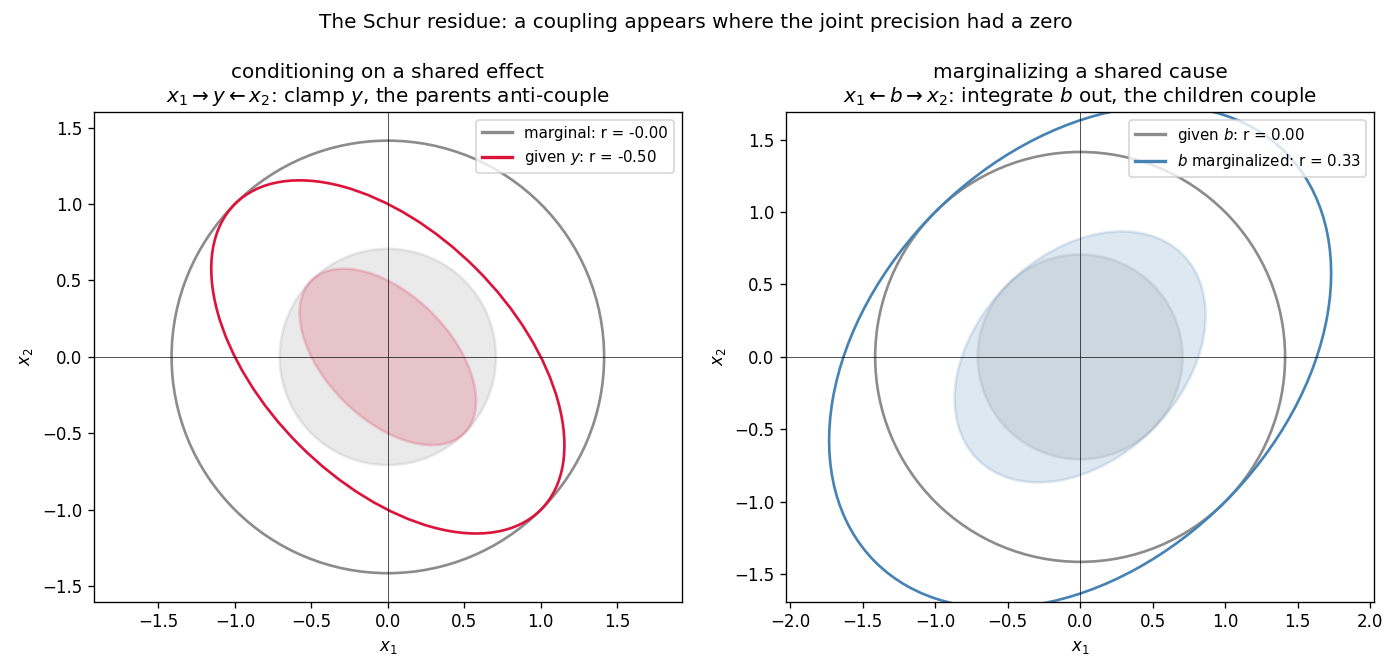
\includegraphics[width=\linewidth]{fig_schur_generic.png}
\caption{The Schur residue, computed on the smallest nets that show it. \emph{Left:} conditioning
on a shared effect ($x_1\!\to\!y\!\leftarrow\!x_2$): the parents are a priori independent (grey,
$r=0$); clamping their common descendant $y$ manufactures an anti-correlation (crimson,
$r=-0.50$)---explaining away. \emph{Right:} marginalizing a shared cause (the matrix of
Eq.~\ref{eq:schur}): the children are independent given $b$ (grey); integrating $b$ out leaves
them coupled (blue, $r=+0.33$). In both cases a coupling appears where the joint precision had a
zero---the off-diagonal mass the carry-over cost $\kappa=\Top\bone$ is built from.}
\label{fig:schur-generic}
\end{figure}

% ======================================================================
\section{The null regime, measured}
\label{app:null}
% ======================================================================

This appendix carries the quantitative characterization of the default (fixed-reliability)
community summarized in \S\ref{sec:res-null}: the full Kuhnian-cycle sweep over the dials of
Table~\ref{tab:dials}, 2{,}488 runs spanning the baseline and every mechanism of
Appendix~\ref{app:closing}.

\begin{table}[h!]
\centering\footnotesize
\begin{tabular}{lll}
\hline
Dial & Symbol & What it controls \\
\hline
Social coupling & \emph{inter} & inter-community trust weight (0 = isolation) \\
Vanguard fraction & --- & fraction of agents in the open (low-$\lambda$) community \\
Conviction & $\lambda_d$ & dogmatic community's value tilt / prune protection \\
Gate scaling & $s$ & strength of the conviction gate on disconfirming channels \\
Proposal rate & $r$ (Poisson) & arrival rate of structural proposals \\
Forgetting & $\omega\in(0,1]$ & decay of accumulated evidence toward the prior \\
Observation noise & $\sigma_o$ & sensory noise at the belt \\
Channel reliability & $\nu$ & Student-$t$ gate on the agent's own channels (off $=$ Gaussian) \\
Social trust & $\nu_s$ & Student-$t$ gate on the fusion weights (off $=$ fixed trust) \\
Fusion protocol & --- & pool all dimensions (delta) vs.\ jointly represented (abstention) \\
Closed-loop mechanisms & $\beta,\tau,\kappa_r,\lambda_c,\epsilon$ & adequacy-driven rate, social
excitation, audit credit, value accretion (Appendix~\ref{app:closing}) \\
\hline
\end{tabular}
\caption{The dials swept in the experiments; all other quantities are held fixed. The last two
rows are protocol and mechanism variations layered on the baseline; each defaults to ``off''
(constant rate, one-shot accept, delta pooling, static $u$, both reliability gates off),
reproducing the baseline model exactly.}
\label{tab:dials}
\end{table}

\paragraph{Only total isolation protects a superseded paradigm.}
The setup pits a dogmatic community---high conviction, whose agents gate their own disconfirming
channels (\S\ref{sec:revision})---against an open vanguard already tracking the anomaly, and
dials the inter-community trust weight \emph{inter} from $0$ (sealed off) to dense contact.
Sealed off, the gating protects: under strong gating ($s=10$) only $19\%$ ever convert. But at
\emph{inter}$=0.005$, $92\%$ convert to oxygen, however strong the gate and however dogmatic the
agents, and the transition is a sharp boundary, not a gradual fade (Fig.~\ref{fig:res-lockin}).
A control pins down what does the stalling: keep conviction exactly as high but switch the
self-gating off, and the community revolts in full (revolted fraction $1.0$ versus $0.0$,
$\gamma\to1$). The tilt never stalls anyone (Eq.~\ref{eq:gamma}); its one causal route to
lock-in runs through the gate, and the gate loses to the faintest connection, because a
neighbour's evidence arrives weighted by trust, not by the receiver's conviction. Motivated
reasoning in this regime is \emph{wishful}, not \emph{dogmatic}: a bias lives in the potential
$h$; an entrenchment would have to live in the precision $\Pi$---which is exactly where the
inferred-reliability gate of \S\ref{sec:reliability} puts it.

\begin{figure}[h!]
\centering
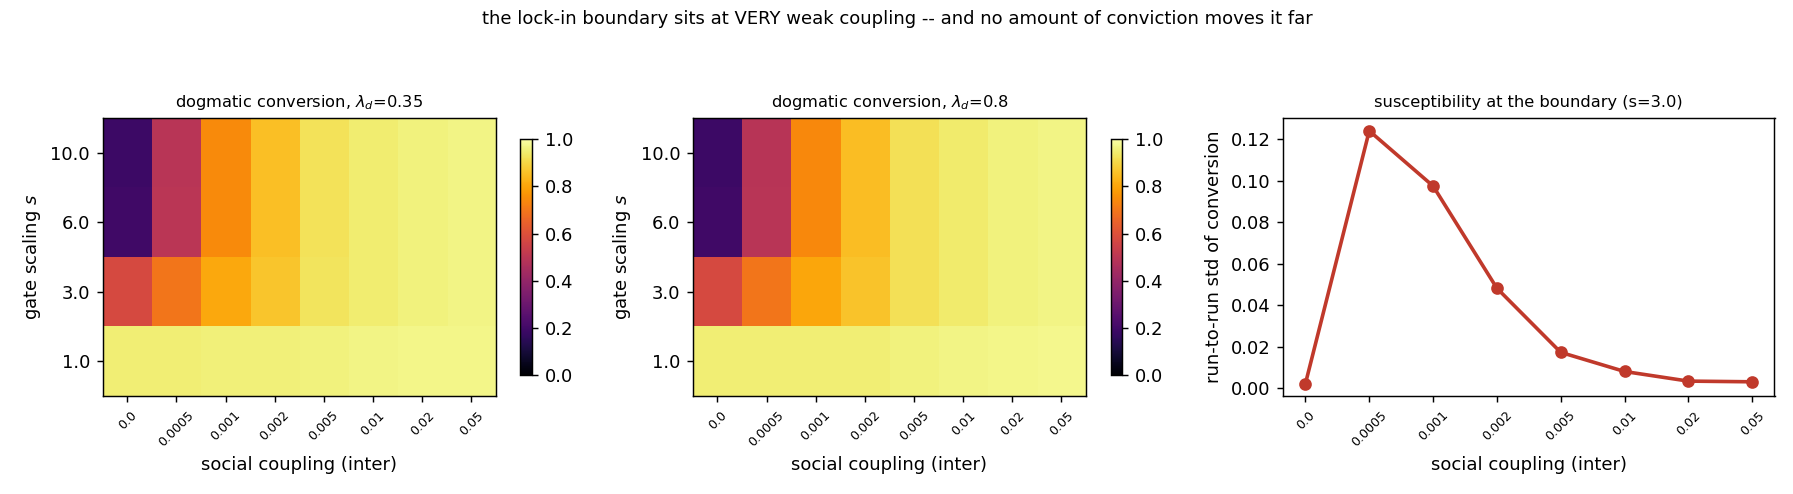
\includegraphics[width=\linewidth]{fig_kuhn_lockin_boundary.png}
\caption{Only isolation protects a superseded paradigm (phlogiston sweep, fixed trust).
\emph{Left, centre:} the fraction of the dogmatic community that converts to oxygen, as a
function of contact (\emph{inter}) and of how strongly conviction gates disconfirming channels
($s$), at two conviction levels ($\lambda_d=0.35$ and $0.8$). Past
\emph{inter}$\,\approx0.005$ nearly everyone converts, and doubling conviction barely changes
the picture. \emph{Right:} the run-to-run spread spikes in a narrow band around
\emph{inter}$\,\approx5\times10^{-4}$: a sharp boundary, not a fade.}
\label{fig:res-lockin}
\end{figure}

\paragraph{Pooling kills the lone discoverer---by protocol, not by principle.}
Discovery means waking a node---oxygen---that no agent's network yet contains; candidates arrive
at random (Poisson rate $r$, \S\ref{sec:structurelearning}), and the fraction that discovers
follows the waiting-time law $1-(1-r)^T$. What the rate governs is survival: under the baseline
fusion, a discovery made by one agent at a time is averaged away every time, because delta
pooling reads \emph{has no such variable}---a fact about an agent's model class---as
\emph{maximally certain it is zero}, a belief within its support
\citep{genest1986,friston2023federated}. The corrected protocol is dimension-aware
\emph{abstention} pooling: each entry of the precision matrix is pooled only over the neighbours
that represent it. The consequence is a wholesale relocation of the survival threshold
(Fig.~\ref{fig:res-fusion}): under delta pooling staggered survival is zero at every rate; under
abstention pooling it tracks the discovery fraction itself ($0.39/0.64/0.86$ at
$r_0=0.005/0.01/0.02$).

\begin{figure}[h!]
\centering
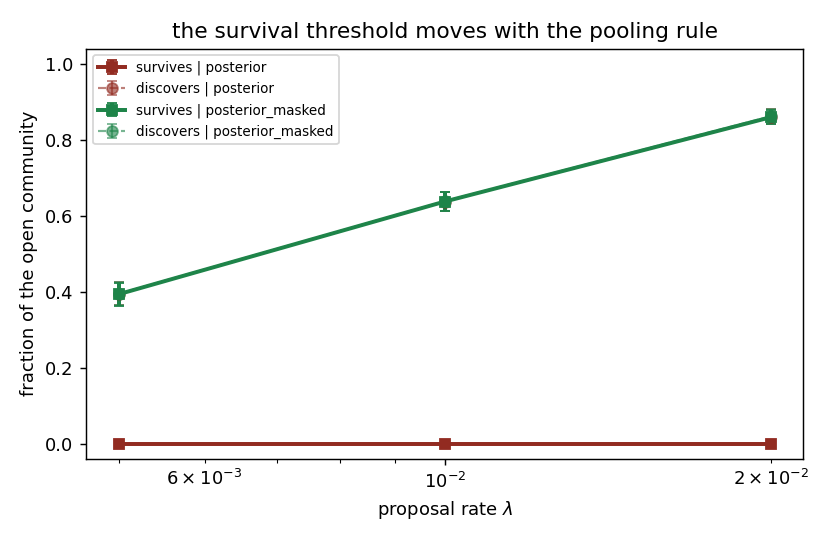
\includegraphics[width=0.62\linewidth]{fig_kuhn_fusion.png}
\caption{The survival threshold moves with the pooling protocol (32 seeds per cell). Solid:
fraction of the open community whose concept survives; dashed: fraction that discovers at all.
Under delta pooling (red) a pinned slot is a confident ``no such thing'' and staggered survival
is zero at every rate; under abstention pooling (green) survival tracks discovery.
Incommensurability as a population-level force is a property of the protocol, not of the
concepts.}
\label{fig:res-fusion}
\end{figure}

\paragraph{Every escape goes around the averaging, never through it.}
The sweep's remaining mechanisms sharpen the same conclusion (Table~\ref{tab:escapes}; full
results in Appendix~\ref{app:closing}). None of them lets two connected communities holding the
same data \emph{remain} in disagreement: each either re-times the passage through the consensus
bottleneck or synchronizes the population for it.

\begin{table}[h!]
\centering\footnotesize
\begin{tabular}{p{0.20\linewidth}p{0.24\linewidth}p{0.30\linewidth}p{0.16\linewidth}}
\hline
Escape & What it changes & Measured effect & Verdict \\
\hline
Adequacy-inferred rate & \emph{when} the community looks & crisis-to-discovery $55\to29$ steps;
matched by a constant rate of equal mean & re-times the passage \\[2pt]
Social excitation (Hawkes) & how nearly \emph{together} it looks & waking dispersion $64\to2$
steps; staggered survival $0\to0.88$--$0.95$ & synchrony outruns the averaging \\[2pt]
Audited wake-then-prune & whether curiosity is \emph{safe} & null world: $100\%$ of wakes
re-pinned, exactly & keeps the search honest \\[2pt]
Value accretion & conviction grown from \emph{inside} & conversion delayed $\sim2.2\times$, never
prevented & buys time, not immunity \\
\hline
\end{tabular}
\caption{Four mechanisms layered on the fixed-reliability baseline, none of which opens the
consensus engine (Appendix~\ref{app:closing}).}
\label{tab:escapes}
\end{table}

\paragraph{Robustness.}
The arc is robust across forgetting and observation noise ($\omega\in[0.9,1.0]$,
$\sigma_o\in[0.25,1.0]$): crisis and reduction survive everywhere---including the no-forgetting
wall $\omega=1$, where only discovery thins: a community that never forgets still sees its
paradigm die, but loses the capacity to grow the successor. Each experiment ships its own null
and positive controls---a world that never shifts produces neither crisis nor discovery; the
gated, isolated community stays locked; Poisson discovery follows the waiting-time law---and no
acceptance bar is tuned anywhere: the wake's sole accept test is the model log Bayes factor
(Appendix~\ref{app:crisis-discovery}); whatever the derivations there do not fix is named there
as a commitment.

% ======================================================================
\section{Inferred reliability: definitions and experiment details}
\label{app:reliability}
% ======================================================================

\paragraph{The three reads of one functional.}
Every gate in the paper is the Student-$t$ scale-mixture weight
$\lambda=(\nu+1)/(\nu+z^2)$---the posterior expectation of a source's latent noise scale given
its standardized squared surprise $z^2$ (one E-step of the EM view of $t$-regression)---applied
to three different surprises. \emph{Channels:} $z_k^2=(o_k-(H\mu)_k)^2/\mathrm{predvar}_k$ with
$\mathrm{predvar}_k=\sigma_o^2+(H\Pi^{-1}H^{\!\top})_{kk}$, the agent's own surprise at
observation $k$ before depositing it; $\lambda_k$ multiplies the channel's deposit, composing
with the conviction gate of \S\ref{sec:revision}. \emph{Opinions:}
$z_{ij}^2=\sum_v(\mu_j[v]-\mu_i[v])^2/(\Pi_i[v,v]^{-1}+\Pi_j[v,v]^{-1})$, the calibrated
disagreement of two posteriors summed over the measured nodes (summed, not averaged: a localized
heresy must be able to sever trust); $\gamma_{ij}$ multiplies the fusion weights, whose row
normalization absorbs the overall scale. \emph{Wiring:} the same sum taken over contested
coupling entries $x=\Pi[a,c]$, normalized by their pairwise symmetric scale
$\max((x_i^2+x_j^2)/2,\,\epsilon^2)$---bounded per coupling, and invariant to the global
precision growth the forgetting equilibrium produces, so it reads \emph{how} two agents wire
the world, not how much evidence they hold. \emph{Edge strain}, the diagnostic of
\S\ref{sec:res-conflict}, is the node-splitting read of the same idea applied to an agent's own
edges: the calibrated displacement between the posterior endpoint marginals with and without an
edge's deposits, a per-step $O(1)$ read of where the model fights the data that ranks candidate
prunes before any Bayes factor is paid.

\paragraph{The experiments.}
Table~\ref{tab:rel-experiments} lists the configurations; all are seeded, assertion-checked at
run time, and write their summary statistics next to their figures.

\begin{table}[h!]
\centering\footnotesize
\begin{tabular}{p{0.23\linewidth}p{0.36\linewidth}p{0.32\linewidth}}
\hline
Experiment & Setup & Headline \\
\hline
Conflict crisis (\S\ref{sec:res-conflict}) & 1 agent, chain $A{\to}B{\to}C$, channel $A$
contradictory from $t{=}30$; $\nu{=}4$, $T{=}120$ & $\lambda_A\!\to\!0.16$; interior variance
maximum at $t{=}38$; strain ratio $5.3{\times}$ on the violated edge \\[2pt]
Targeted reduction (\S\ref{sec:res-conflict}) & 1 agent, chain with one world-violated coupling,
$T{=}80$ & violated edge top-strain at $100\%$ of steps; $\Delta F$ verdicts correct from step
1 \\[2pt]
Crisis trace (\S\ref{sec:res-crisis}) & $N{=}20$, flip at $t{=}40$, $\nu{=}2$, $T{=}800$ &
denial $\bar\lambda\,{:}\,0.85\!\to\!0.17$; stall $4.3{\times}$; rehabilitation to $1.27$;
agreement channels $>0.85$ throughout \\[2pt]
Gated camps & $N{=}20$, complete graph, opposed camps, $\nu_s{=}0.5$, $T{=}80$ & uniform fusion:
$0.1\%$ of disagreement survives; gated: $48\%$; cross/within trust $0.8\%$ \\[2pt]
Schism threshold (\S\ref{sec:res-schools}) & ditto, sweeping prior confidence at contact &
fixed trust $\le0.2\%$ everywhere; gated $<1\%$ below the threshold, $17/48/76\%$ above \\[2pt]
Lock-in rerun (\S\ref{sec:res-schools}) & $N{=}80$, full cycle, $\nu_s{=}0.5$, $T{=}180$,
\emph{inter} swept & $t_{1/2}$: $78\!\to\!146$--$170$ at the boundary; conversion $0.54$--$0.73$
vs $0.92$; trust $<1\%$ then $>90\%$ \\[2pt]
Divergent wiring (\S\ref{sec:res-pluralism}) & $N{=}60$, structurally underdetermined world, two
attention camps, $T{=}120$, 5 seeds & retention: fixed $10\%$, opinion-gate $10.2\%$,
wiring-gate $94\%$; synergy $=0$ \\
\hline
\end{tabular}
\caption{The gated experiments: configurations and headline numbers.}
\label{tab:rel-experiments}
\end{table}

\paragraph{Scope, stated plainly.}
Three commitments bound the results. (i) Both gates are \emph{memoryless}: $\lambda$ and
$\gamma$ are instantaneous functions of current surprise, so every school and schism reported is
metastability relative to a horizon, not a new fixed point---the contraction theorem owns
$t\to\infty$, and the lock-in rerun shows the trade directly: a harsher gate ($\nu_s{=}0.2$)
holds the boundary longer but leaves the rehabilitation arc unfinished at the same horizon,
because the lock and the merge run on the same clock. (ii) The schism control is normalized by
the pre-contact stance gap, since one uniform fusion step collapses the fixed-trust camps before
the first logged sample. (iii) Structure-as-precision-pattern is attention-driven in the
linear-Gaussian class (the Fisher deposit $H^{\!\top}\mathrm{diag}(w)H/\sigma^2$ never sees the
observation's value), which is what refuted the three-camps prediction of
\S\ref{sec:res-pluralism} and is the right caveat on every wiring-gate claim.

% ======================================================================
% The crisis and discovery checks, derived from the ledger (+ the
% exploration-as-social-process mechanism readings at its tail).
\input{appendix_crisis_discovery_v4}

% ======================================================================
\section{Closed-loop mechanisms: quantitative results}
\label{app:closing}
% ======================================================================

The baseline model holds four quantities fixed that admit treatment as beliefs or protocols: the
proposal rate, the acceptance of a wake, the conviction source $u$, and the pooling rule. The
inferential readings that license each mechanism are derived in
Appendix~\ref{app:exploration-future}; this appendix reports what each does to the population
results. Every mechanism defaults to ``off''---constant rate, one-shot accept, static $u$, delta
pooling---reproducing the baseline exactly, and each comparison below is run against that
baseline with its own control.

\paragraph{The rate as a posterior over model adequacy.}
The agent tracks its residual floor---the leading eigenvalue of the windowed prediction-error
second moment, the error no within-model update can absorb---with a fixed-gain filter
$s \leftarrow (1-\rho)\,s + \rho\cdot\mathrm{floor}$ and reads its proposal rate off the
posterior, $r(t) = r_0 + \kappa_r \max(s - s_{\mathrm{ref}}, 0)$. The result
(Fig.~\ref{fig:res-rateposterior}) has the signature a posterior should have and a dial cannot:
flat at $r_0$ through normal science, surging after the agent's own crisis exposes the residual
(to an effective $0.34$ from $r_0=0.01$), and decaying once the woken node explains it. The
crisis-to-discovery delay falls from $55$ to $29$ steps---but the control that matters is the
fixed rate it \emph{matches}: a constant-rate agent given the adaptive run's realized mean rate
achieves the same delay ($27$ steps). The gain is not more exploration; it is exploration when
the agent's own evidence calls for it. Stanford's constraint survives: only the \emph{propensity
to look} is inferred, never a direction.

\begin{figure}[h!]
\centering
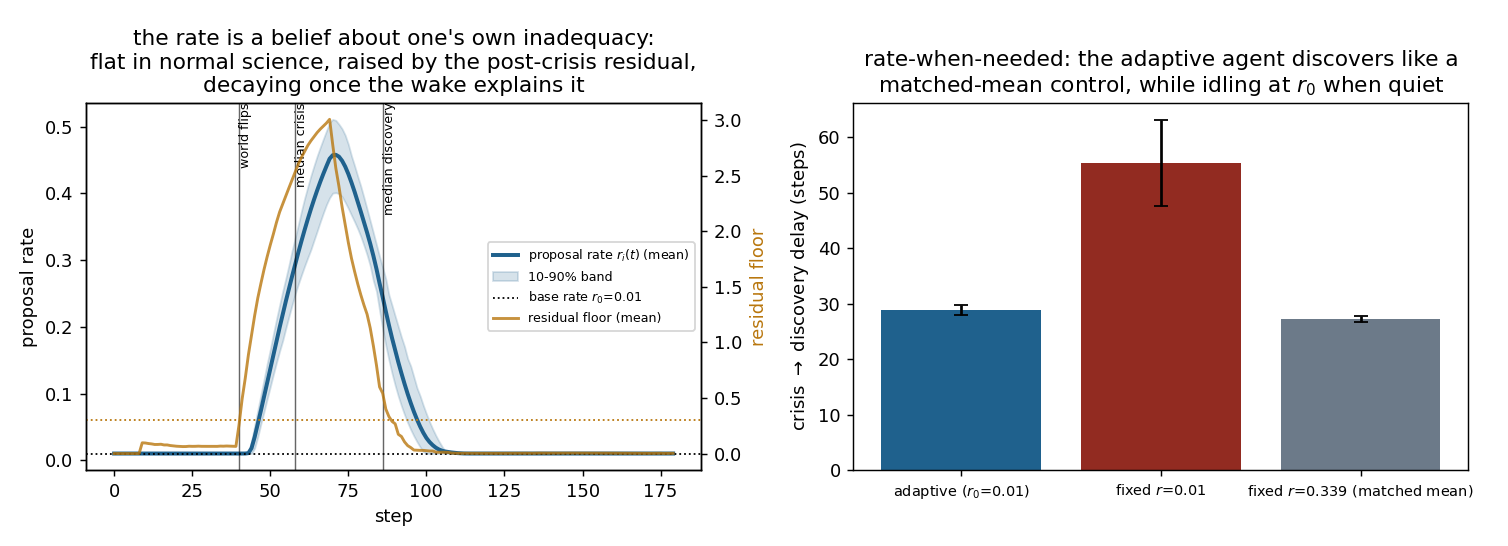
\includegraphics[width=\linewidth]{fig_rate_posterior.png}
\caption{The proposal rate as a posterior over model adequacy. \emph{Left:} the per-agent rate
(blue, mean and 10--90\% band) is flat at the base rate $r_0$ through normal science, rises with
the post-crisis residual floor (amber, right axis)---the evidence of model-class inadequacy the
within-model updates cannot absorb---and decays once the woken node explains it. \emph{Right:}
crisis-to-discovery delay. The adaptive agent (left bar) matches a fixed-rate control given its
realized mean rate (right bar) while idling at $r_0$ when the model is adequate: the gain is
rate-when-needed, not more rate.}
\label{fig:res-rateposterior}
\end{figure}

\paragraph{Social excitation rescues the staggered discovery.}
Filtering neighbours' discovery events through the trust weights, under an
exponentially-correlated prior on the latent inadequacy, yields a posterior intensity of exactly
the linear self-exciting (Hawkes) form \citep{hawkes1971},
\begin{equation}
r_i(t) \;=\; r_0 \;+\; \sum_{j\in\partial i} T_{ij} \sum_{t_j<t} \beta\, e^{-(t-t_j)/\tau},
\label{eq:hawkes}
\end{equation}
with $t_j$ the neighbours' discovery times, $\beta$ the trust-scaled evidential weight of one
observed discovery, and $\tau$ the assumed correlation time of inadequacy
(Appendix~\ref{app:exploration-future}). Under Eq.~\eqref{eq:hawkes} the first discovery raises
the whole neighbourhood's propensity to look; the cascade compresses the community's wakings from
a dispersion of $64$ steps to $2$, and---because survival is \emph{completeness}-driven (a single
still-pinned peer holds the fused slot precision enormous for every neighbour)---the completed
cascade lets the anchored couplings consolidate. Survival rises monotonically in $\beta$ from
exactly zero at $\beta=0$ to $0.88$--$0.95$ at $\beta=1.5$ across base rates
$r_0\in\{0.005,0.01,0.02\}$ at which an unexcited community essentially never completes
(Fig.~\ref{fig:res-hawkes}; 32 seeds per cell). The branching ratio of Eq.~\eqref{eq:hawkes} is
the model's quantitative answer to how much social excitement a revolution needs. One qualifier:
survival is completeness-driven and therefore horizon-bound---a constant-rate community given a
high enough rate and a long enough horizon also completes its cascade; what excitation adds is
the mechanism by which a community reaches near-simultaneity at rates serendipity alone
essentially never does.

\begin{figure}[h!]
\centering
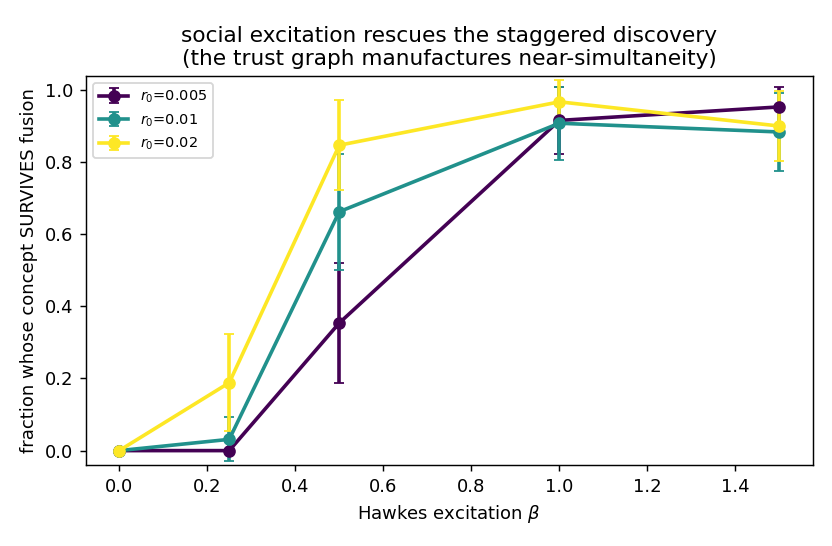
\includegraphics[width=0.62\linewidth]{fig_kuhn_hawkes.png}
\caption{Social excitation rescues the staggered discovery (sweep panel E, 32 seeds per cell).
Fraction of the open community whose oxygen concept survives fusion, versus the excitation
$\beta$ of Eq.~\eqref{eq:hawkes}, at three base rates. At $\beta=0$ (the constant rate) survival
is exactly zero: staggered wakings are crushed one at a time. Excitation compresses the
community's wakings in time, the cascade completes, no pinned peer remains in the fusion average,
and survival rises to $0.88$--$0.95$---the near-simultaneity that survival requires, manufactured
by the community itself.}
\label{fig:res-hawkes}
\end{figure}

\paragraph{The audited wake-then-prune cycle.}
Accepting wakes on the full ledger $\Delta F + \Delta G > 0$ lets curiosity adopt structure the
data do not yet hold, and the audit of Appendix~\ref{app:exploration-future} pays that debt: in a
null world that never shifts, curiosity wakes structure in $100\%$ of agents and the audit
re-pins $100\%$ of those wakes, exactly; in the flip world the genuine hub is woken everywhere
and never pruned (Fig.~\ref{fig:wakeprune}). Two companion measurements close two more
commitments. Widening the search---three eigen-hub candidates, each with its own dormant slot,
plus the three largest residual couplings, $1{,}140$ candidates priced on the same ledger---does
not dilute discovery: the true cause wins $53$ of $60$ acceptances (median cosine $0.999$ against
the rank-one baseline). And running the identical discovery check \emph{before} each agent's
crisis, at every step, the ledger rejects $13{,}180$ of $13{,}185$ pre-crisis agent-steps: the
crisis-before-expansion ordering is enforced by the evidence, not by fiat---the intact paradigm
absorbs the residual, so there is nothing for the check to find until reduction exposes it.

\paragraph{Value accretion (Lakatos, run forward).}
Letting $u$ accrete onto the commitments the agent's own evidence deposit has entrenched
(Appendix~\ref{app:exploration-future}) closes the loop through the gate of
Eq.~\eqref{eq:gamma}: a maturing programme increasingly silences its own disconfirming channels
($\gamma$ climbs from $0.72$ to $0.97$ as $\epsilon$ rises), conversion at the lock-in boundary
falls from $0.94$ to $0.67$, and at very weak coupling the dogmatic community's conversion is
\emph{delayed} roughly $2.2$-fold rather than prevented (Fig.~\ref{fig:lakatos}). Conviction that
grows from the inside still loses to connection: it buys the old paradigm time, not immunity---a
fair gloss of a degenerating problemshift.

\paragraph{The mechanisms compose.}
With the adequacy-posterior rate, social excitation, the expiring-credit audit, abstention
pooling and value accretion all enabled in one population, the full arc still runs---crisis at
$t\approx67$, discovery at $t\approx69$, the rate surging $0.02\to0.77$ and decaying back to
base, zero false prune-backs, concept survival complete, and the never-shifting null world silent
in every channel. No mechanism breaks another, because none adds a new objective: each routes a
quantity the ledger already computes---residual, epistemic gain, evidence, deposit---back into a
parameter that had been a constant.

\end{document}
